%\documentclass[letterpaper]{IEEEtran}
\documentclass[letterpaper, 11pt]{IEEEtran}      % Use this line for a4 paper

%LatexiDiff ignore tikz:
% $: latexdiff -c "PICTUREENV=(?:picture|tikzpicture|DIFnomarkup)[\w\d*@]*" old.tex new.tex > diff.tex

%\IEEEoverridecommandlockouts                              %

%\usepackage{mathcomSTEP}

%\overrideIEEEmargins 
%\IEEEoverridecommandlockouts                              % This command is only needed if 
% you want to use the \thanks command

%\overrideIEEEmargins                                      % Needed to meet printer requirements.

% See the \addtolength command later in the file to balance the column lengths
% on the last page of the document

\onecolumn

\usepackage{mathptmx} 
\usepackage{times} 
\usepackage{amsmath} 
\usepackage{amsbsy} 
\usepackage{amssymb}
%\usepackage{newtxtext, newtxmath}
\usepackage{mathrsfs}
\usepackage{comment}
\usepackage[export]{adjustbox}
\usepackage{tikz}
\usetikzlibrary{external,positioning,decorations.pathreplacing,shapes,arrows,patterns}

%\tikzexternalize[mode=list and make]
\usepackage{algorithmicx}
\usepackage{pgfplots}
\usepackage{graphicx}
\usepackage{pstool}
\usepackage[latin1]{inputenc}
\usetikzlibrary{arrows,shapes}
\usepackage{xifthen}
\usepackage{epic}
%\usepackage{caption}
\usepackage{epstopdf}

\newtheorem{thm}{\bf{Theorem}}
\newtheorem{cor}[thm]{\bf {Corollary}}
\newtheorem{lem}[thm]{\bf {Lemma}}
\newtheorem{prop}[thm]{\bf {Proposition}}
\newtheorem{example}{\bf {Example}}
\newtheorem{definition}{\bf {Definition}}
\newtheorem{rem}{\bf {Remark}}
\newtheorem{assump}{\bf {Assumptions}}

\newcommand{\mmse}{\mathsf{mmse}}
\newcommand{\unif}{\mathsf{unif}}
\newcommand{\card}{\mathrm{card}}
\newcommand{\ARE}{\mathsf{ARE}}
\newcommand{\supp}{\mathrm{supp} }
\renewcommand\vec[1]{\ensuremath\boldsymbol{#1}}
\newenvironment{proof}{\paragraph*{Proof}}{\hfill$\square$ \newline}
\newcommand{\sgn}{\mathrm{sgn} }
\newcommand{\Prob}{\mathbb{P} }
\newcommand{\argmax}{\mathrm{argmax}}
\newcommand*{\QEDA}{\hfill\ensuremath{\square}}



\tikzstyle{int}=[draw, fill=blue!10, minimum height = 1cm, minimum width=1.5cm,thick ]
\tikzstyle{sint}=[draw, fill=blue!10, minimum height = 0.5cm, minimum width=0.8cm,thick ]
\tikzstyle{sum}=[circle, fill=blue!10, draw=black,line width=1pt,minimum size = 0.5cm, thick ]
\tikzstyle{ssum}=[circle, fill=blue!10,draw=black,line width=1pt,minimum size = 0.1cm]
\tikzstyle{int1}=[draw, fill=blue!10, minimum height = 0.5cm, minimum width=1cm,thick ]
\tikzstyle{enc}=[draw, fill=blue!10, minimum height = 2.7cm, minimum width=1cm,thick ]
\tikzstyle{int}=[draw, fill=blue!10, minimum height = 1cm, minimum width=1.5cm,thick ]


\author{
    \IEEEauthorblockN{John C. Duchi\IEEEauthorrefmark{1}\IEEEauthorrefmark{2} and
Alon Kipnis\IEEEauthorrefmark{1} \\}
    \IEEEauthorblockA{\IEEEauthorrefmark{1}Stanford University, Department of Statistics \\}
    \IEEEauthorblockA{\IEEEauthorrefmark{2}Stanford University, Department of Electrical Engineering. }
}

\title{\LARGE \bf Mean Estimation from One-Bit Measurements}


\begin{document}
\graphicspath{{./Figs/}}
\maketitle
\thispagestyle{empty}
\pagestyle{empty}


%%%%%%%%%%%%%%%%%%%%%%%%%%%%%%%%%%%%%%%%%%%%%%%%%%%%%%%%%%%%%%%%%%%%%%%%%%%%%%%%
\begin{abstract}
We consider the problem of estimating the mean of a symmetric log-concave distribution under the following constraint: only a single bit per sample from this distribution is available to the estimator. We study the mean squared error (MSE) risk in this estimation as a function of the number of samples, and hence the number of bits, from this distribution. Under an adaptive setting in which each bit is a function of the current sample and the previously observed bits, we show that the optimal relative efficiency compared to the sample mean is the efficiency of the median. For example, in estimating the mean of a normal distribution, a constraint of one bit per sample incurs a penalty of $\pi/2$ in sample size compared to the unconstrained case. 
%
We also consider a distributed setting where each one-bit message is only a function of a single sample. We derive lower bounds on the MSE in this setting, and show that the optimal efficiency can only be attained at a finite number of points in the parameter space. 
%
Finally, we analyze a distributed setting where the bits are obtained by comparing each sample against a prescribed threshold. Consequently, we consider the threshold density that minimizes the maximal MSE. 
%
Our results indicate that estimating the mean from one-bit measurements is equivalent to estimating the sample median from these measurements. In the adaptive case, this estimate can be done with vanishing error for any point in the parameter space. In the distributed case, this estimate can be done with vanishing error only for a finite number of possible values for the unknown mean. 
%
%Therefore, our results indicate that, rather surprisingly, parametric estimation from the coarsest form of quantization incurs only a multiplicative penalty factor on the number of measurements. For example, this factor is $\pi/2$ for the normal distribution. 
\end{abstract}

%{\color{red}  See LASSO results in http://arxiv.org/abs/1506.02181v1}


%%%%%%%%%%%%%%%%%%%%%%%%%%%%%%%%%%%%%%%%%%%%%%%%%%%%%%%%%%%%%%%%%%%%%%%%%%%%%%%%
\section{Introduction}
\label{sec:Intro}
Estimating parameters from data collected and processed by multiple units may be limited due to communication constraints between these units. 
%
For example, this scenario arises in sensor arrays where information is collected at multiple physical locations and transmitted to a central estimation unit. In these situations, the ability to estimate a particular parameter from the data is dictated not only by the quality of observations and their number but also by the available bandwidth for communicating between the sensors and the central estimator. The question that we ask is to what extent a parametric estimation task is affected by this constraint on communication, and what are the fundamental performance limits in estimating a parameter subject to such restriction. \par
This paper answers this question in a particular setting: the estimation of the mean $\theta$ of a symmetric log-concave distribution with finite variance, under the constraint that only a single bit can be communicated on each sample from this distribution. As it turns out, the ability to share information before committing on each one-bit message dramatically affects the performance in estimating $\theta$. We, therefore, distinguish among three settings:
\begin{itemize}
 \item[(i)\,\,] \emph{Centralized} encoding (Fig.~\ref{fig:centralized}): all $n$ encoders confer and produce a single $n$ bit message. 
 \item[(ii)\,] \emph{Adaptive} or \emph{sequential} encoding (Fig.~\ref{fig:sequential}): the $n$th encoder observes the $n$th sample and the $n-1$ previous messages (bits).
 \item[(iii)] \emph{Distributed} encoding (Fig.~\ref{fig:distributed}): the $n$th message is only a function of the $n$th observation.
 \end{itemize}
Evidently, as far as information sharing is concerned, settings (iii) is a more restrictive version of (ii) which is more restrictive than (i). Below are three application examples for each of settings (i)-(iii) above, respectively:
\begin{itemize}
\item {\bf Signal acquisition:} a quantity is measured $n$ times at different instances, and the results are averaged in order to reduce measurement noise. The averaged result is then stored using one of $n$ states. 
\item {\bf Analog-to-digital conversion:} A sigma-delta modulator (SDM) converts an analog signal into a sequence of bits by sampling the signal at a very high rate and then using one-bit threshold detector combined with a feedback loop to update an accumulated error state \cite{1092194}. Therefore, the MSE in tracking an analog signal using a SDM falls under our setting (ii) when we assume that the signal at the input to the modulator is a constant (direct current) corrupted by, say, thermal noise \cite{53738}. Since the sampling rates in SDM are usually many times more than the bandwidth of its input, analyzing SDM under a constant input provides meaningful lower bound even for non-constant signals.
\item {\bf Differential privacy:} -- a business entity is interested in estimating the average income of its clients. In order to keep this information as confidential as possible, each client independently provides an answer to a yes/no question related to its income.
\end{itemize}
%
We measure the performance in estimating $\theta$ by the mean squared error (MSE) risk. We are interested in particular in the \emph{asymptotic relative efficiency} (ARE) of estimators in the constrained setting compared to asymptotically normal estimators whose variances decreases as $\sigma^2/n+o(n^{-1})$. Estimators of this form include the empirical mean of the samples, and, under some conditions, the optimal Bayes estimator. \par
%
In addition to the examples above, the excess risk in estimating a fixed parameter due to a one-bit per measurement constraint is useful in bounding from below the excess risk in estimating a signal from its noisy measurements. Namely, the excess MSE or ARE we derive serves as the most optimistic estimate for the risk in estimating under the one-bit per measurement constraint a signal changing over time or space. Such estimation settings are considered in \cite{baraniuk2017exponential, jacques2013robust, plan2013one, li2017channel, choi2016near}. \\


% given a prior distribution on the space $\Theta$ where $\theta$ resides. \\

In setting (i), the estimator can evaluate the optimal mean estimator (e.g., the sample mean in the Gaussian case) and then quantize it using $n$ bits. Since the accuracy in describing the empirical mean decreases exponentially in $n$, the error due to quantization is negligible compared to the MSE in estimating the mean. Therefore, the ARE in this setting is $1$. Namely, asymptotically, there is no loss in performance due to the communication constraint under centralized encoding. 
%
In this paper we show that a similar result does not hold in setting (ii): the ARE of any adaptive estimation scheme is at most the ARE of the sample median. Specifically, when the samples are drawn from the normal distribution, this ARE equals $\pi/2$, showing that the one-bit constraint increases the effective sample size in estimating $\theta$ by at least $\pi/2 \approx 1.57$ compared to estimating it without the bit constraint. We also show that this lower bound on the ARE is tight by providing an estimator that attains it. % This estimator is obtained by averaging the results of a series of comparisons of the samples against certain thresholds. 
%This estimator is can be seen as a stochastic gradient descent procedure for minimizing the absolute error, hence it attains the asymptotic MSE of the sample median. % Interestingly, our estimator attains \eqref{eq:median_MSE} regardless of the particular realization of $\theta$ or the radius of the parameter space from which it is taken.
%
Clearly, the penalty on the sample size in setting (iii) is at least as large as that in setting (ii). Furthermore, we show that, unlike in setting (ii), there is no distributed estimation scheme that is uniformly optimal in the sense that it attains the ARE of the sample median for all $\theta$ in the parameter space. 
% Instead, in setting (iii) we restrict ourselves to estimators from messages obtained by comparison against a prescribed value (that may be different for each sample). We show that the maximum likelihood (ML) estimator for $\theta$ from these messages is asymptotically local minimax, and its asymptotic variance is strictly greater than the variance of the median. Thus, at least when limited to threshold detection, the ability to adapt the threshold allows for a more efficient estimation. %This is in contrast to the \\ counterpart of our setting where $\theta$ is taken from a finite space 

We note that although the ARE in setting (i) is $1$, this scheme already poses a non-trivial challenge for the design and analysis of an optimal encoding and estimation procedures. Indeed, the standard technique to encode an unknown random quantity using $n$ bits is equivalent to the design of a scalar quantizer \cite{gray1998quantization}. However, the optimal design of this quantizer depends on the distribution of its input, which is the goal of our estimation problem and hence its exact value is unknown. As a result, a non-trivial exploration-exploitation trade-off arises in this case. 
%Note that the only missing parameter in our setting is the mean, which, under setting (i), is known to the encoder with uncertainty interval proportional to $\sigma/\sqrt{n}$. 
Therefore, while uncertainty due to quantization decreases exponentially in the number of bits $n$, hence the ARE is $1$, an exact expression for the MSE in this setting is still difficult to derive. \par
%
The situation is even more involved in the adaptive encoding setting (ii): an encoding and estimation strategy that is optimal for $n-1$ adaptive one-bit messages of a sample of size $n-1$ may not lead to a globally optimal strategy upon the recipient of the $n$th sample. Conversely, any one-step optimal strategy, in the sense that it finds the best one-bit message as a function of the current sample and the previous $n-1$ messages, is not guaranteed to be globally optimal. Therefore, while we characterize the optimal one-bit message given the previous messages, this characterization does not necessarily lead to an upper bound on the ARE. Instead, our result on the maximal ARE is obtained by bounding the Fisher information of any $n$ adaptive messages and using an appropriate information inequality. \par
In addition to encoding and estimation schemes that lead to optimal results, we also consider two additional ``natural'' schemes. Specifically, in setting (ii) we consider the one-bit optimal scheme, i.e., the case of a greedy encoder that given the $n$th sample and the previous $n-1$ bits, provides a bit that minimizes the $n$-step MSE. In setting (iii) we also consider the case where the messages are obtained by comparing each sample against a prescribed threshold. This threshold may be different across samples and is assumed deterministic (independent of the data). 

%Finally, we show that an estimator that attains asymptotic MSE of $\sigma^2\pi/(2n)$ is obtained as a special case of \cite[Thm. 4]{polyak1992acceleration}. In addition to these two results, we also derive the one-step optimal strategy in which the message sent at step $i$th is designed to minimize the MSE given this message and the previous $i-1$ messages. Furthermore, we demonstrate numerically that the MSE under this strategy converges to $\pi \sigma^2/(2n)$.\\ 


\subsection*{Related Works}
As the variance $\sigma^2$ goes to zero, the task of finding $\theta$ using one-bit queries in the adaptive setting (ii) is solved by a bisection style method over the parameter space. Therefore, the general case of non-zero variance is reminiscent of the noisy binary search problem with a possibly infinite number of unreliable tests \cite{cicalese2002least, Karp:2007:NBS:1283383.1283478}. However, since we assume a continuous parameter space, a more closely related problem is that of one-bit analog-to-digital conversion of a constant input corrupted by Gaussian noise. Using an SDM, Wong and Gray \cite{53738} showed that the output of the modulator converges to the true constant input almost surely, so that an SDM provides a consistent estimator for setting (ii). The rate of this convergence, however, was not analyzed and cannot be derived from the results of \cite{53738}. In particular, our results for setting (ii) imply that the asymptotic rate of convergence of the MSE in SDM to a constant input under an additive white Gaussian noise is at most $\sigma^2\pi/2$ over the number of feedback iterations. Baraniuk et. al \cite{baraniuk2017exponential} also considered adaptive one-bit measurements in the context of analog-to-digital conversion, although without noise at the input. By establishing the lower bound of $\sigma^2\pi/2n$ on the MSE, we show that the main results of \cite{baraniuk2017exponential}, an exponential MSE decaying rate, does not hold in the noisy setting. Stated otherwise, the MSE in the setting of \cite{baraniuk2017exponential} may decay exponentially up to the noise level, after which it decays at most as $\sigma^2\pi/2n$. \par
%
One-bit measurements in the distributed setting (iii) was considered in \cite{904560,4244748, 6882252, chen2010performance, 5184907}, but without optimizing the encoders and their detection rules. Consequently, the performance derived in these works are not optimal. 
 % analyzed the estimation from distributed quantized measurements when the same detection rule is applied by all encoders. However, the error criterion considered in these works is the Fisher information rather than the MSE risk or ARE criterion. \par
%Once the decision rule of each encoder is fixed, the optimal estimation of $\theta$ is determined using the maximum a posteriori probability rule. Hence, the distributed setting is reduced to finding the optimal decision rule of each encoder.
The work of \cite{52470} addresses the counterpart of our setting (iii) in the case of hypothesis testing, although the results there cannot be extended to parametric estimation. When the parameter space $\Theta$ is finite, Tsitsiklist \cite{tsitsiklis1988decentralized} showed that when the cardinality of $\Theta$ is at most $M$ and the probability of error criterion is used, then no more than $M(M-1)/2$ different detection rules are necessary in order to attain probability of error decreasing exponentially with the optimal exponent. %That is, beyond $M(M-1)/2$ some decision rules can be repeated without losing optimality.
Furthermore, in a version of this problem for the adaptive setting \cite{5751320}, it was shown that, with specific two-stage feedback, there is no gain in feedback compared to the fully distributed setting. Our results imply that they ARE in the distributed setting with threshold detection rules is strictly larger than that in the adaptive setting, suggesting that the case of a finite $\Theta$ is very different from the case where $\Theta$ is an open set.\par
%
As we explain in detail in Section~ \ref{sec:preliminary}, the remote multiterminal source coding problem, also known as the CEO problem \cite{berger1996ceo, viswanathan1997quadratic, oohama1998rate, prabhakaran2004rate}, leads to lower bounds on the MSE in setting (iii). For the case of a Gaussian distribution, this lower bound bounds the ARE to be at most $3/4$. Thus, while this bound on the ARE provides no new information compared to the upper bound of $2/\pi$ we derive for setting (ii), it shows that the distributed nature of the problem is not a limiting factor in achieving MSE close to optimal even under the one bit per sample constraint. 
 \par
% 
Finally, we note that our settings (ii) and (iii) can be obtained as special cases of 
\cite{zhang2013information} 
that consider adaptive and distributed estimation protocols for $m$ machines, each has access to $n/m$ independent samples. The main result of \cite{zhang2013information} are bounds on the estimation error as a function of the number of bits $R$ each machine uses for communication. The specialization of their result to our setting, by taking $m=n$ and $R=1$, leads to looser lower bounds then the ones we derive in this paper for cases (ii) and (iii). Looser bounds can also be obtained from works considering general inference and distributed estimation problems under data compression constraint \cite{DBLP:journals/corr/abs-1802-08417, zhang1988estimation, han2018distributed, xu2017information}. \\
%in MIMO detection in wireless communication \cite{singh2009limits}. \\

The remainder of this paper is organized as follows. In Section~\ref{sec:problem} we describe the problem and useful notation. In Section~\ref{sec:preliminary} we provide two simple bounds on the efficiency and MSE. Our main results for the adaptive and distributed cases are given in Sections~\ref{sec:sequential} and \ref{sec:distributed}, respectively. In Section~\ref{sec:conclusions} we provide concluding remarks. 

\section{Problem Formulation \label{sec:problem}}

\begin{figure}
\begin{center}
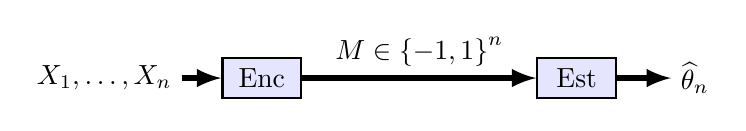
\begin{tikzpicture}[node distance=2cm,auto,>=latex]

\node[node distance = 1.5cm] at (0,0) (source2) {$X_1,\ldots,X_n$};
\node[int1, right of = source2, node distance = 2cm] (enc2) {Enc};  
\draw[->,line width = 2pt] (source2) -- (enc2); 
\node[int1, right of = enc2, node distance = 4cm ] (est) {Est};

\draw[->,line width = 2pt] (enc2) -- node[above, xshift = 0cm] (mes2) {$M \in \left\{-1,1\right\}^n$} (est);   

\node[right of = est, node distance = 1.5cm] (dest) {$\widehat{\theta}_n$};
%         \node [int1] (dec) [right of=dest, node distance = 1.5cm,  align=center] {\small Dec };
%\node [int1] (enc) [right of = dec, node distance = 3cm]{Enc}; 
%\draw[->,line width=2pt] (dec) -- (dest);
\draw[->, line width=2pt] (est) -- (dest);
\end{tikzpicture}
\end{center}
\caption{\label{fig:centralized} Centralized one-bit encoding: encoder sends $n$ bits after observing $n$ samples.}
\end{figure}


\begin{figure}
\begin{center}
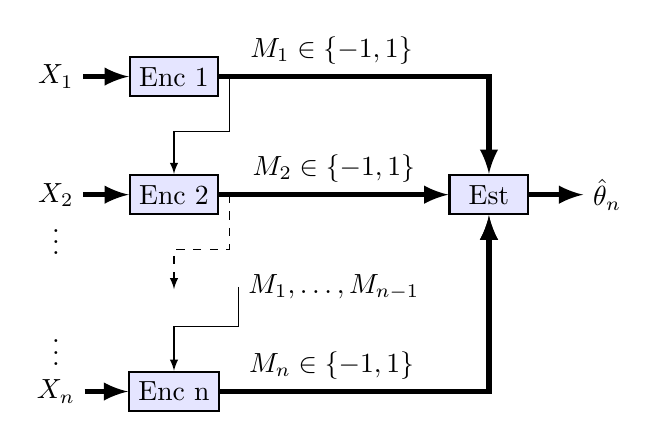
\begin{tikzpicture}[node distance=2cm,auto,>=latex]
  \node at (0,0) (source) {$X_1$} ;
  \node[int1, right of = source, node distance = 1.5cm] (enc1) {Enc 1};  
\draw[->,line width = 2pt] (source) -- (enc1); 

 \node[below of = source, node distance = 1.5cm] (source2) {$X_2$};
\node[int1, right of = source2, node distance = 1.5cm] (enc2) {Enc 2};  
\draw[->,line width = 2pt] (source2) -- (enc2); 

\node[below of = source2, node distance = 2.5cm] (source3) {$X_n$};
\node[int1, right of = source3, node distance = 1.5cm] (enc3) {Enc n};  
\draw[->,line width = 2pt] (source3) -- (enc3); 

\node[below of = source2, node distance = 0.5cm] {$\vdots$};
\node[above of = source3, node distance = 0.6cm] {$\vdots$};
%\node[above of = source3, node distance = 1cm] (dist) {$X_i \sim P_X$};

\node[int1, right of = enc2, node distance = 4cm ] (est) {Est};
\draw[->,line width = 2pt] (enc1) -| node[above, xshift = -2cm] (mes1) {$M_1 \in \left\{-1,1\right\}$} (est);   
\draw[->,line width = 2pt] (enc2) -- node[above, xshift = 0cm] (mes2) {$M_2 \in \left\{-1,1\right\}$} (est);   

\draw[->] (enc1)+(0.7,0) -- +(0.7,-0.7) -| (enc2);

\draw[dashed,->] (enc2)+(0.7,0) -- +(0.7,-0.7) -| +(0,-1.2);
\draw[->,line width = 2pt] (enc3) -| (est);   

\node[below of = mes2, node distance = 1.5cm] (mes3) {$M_1,\ldots,M_{n-1} $};

\draw[->,line width = 2pt] (enc3) -| node[above, xshift = -2cm]  {$M_n \in \left\{-1,1\right\}$} (est);   

\draw[->] (mes3.west) -- +(0,-0.5) -| (enc3);

\node[right of = est, node distance = 1.5cm] (dest) {$\hat{\theta}_n$};
%         \node [int1] (dec) [right of=dest, node distance = 1.5cm,  align=center] {\small Dec };
%\node [int1] (enc) [right of = dec, node distance = 3cm]{Enc}; 
%\draw[->,line width=2pt] (dec) -- (dest);
\draw[->, line width=2pt] (est) -- (dest);
\end{tikzpicture}
\end{center}
\caption{\label{fig:sequential} Adaptive one-bit encoding: the $n$th encoder delivers a single bit message which is a function of its private sample $X_n$ and the previous messages $M_1,\ldots,M_{n-1}$.}
\end{figure}


\begin{figure}
\begin{center}
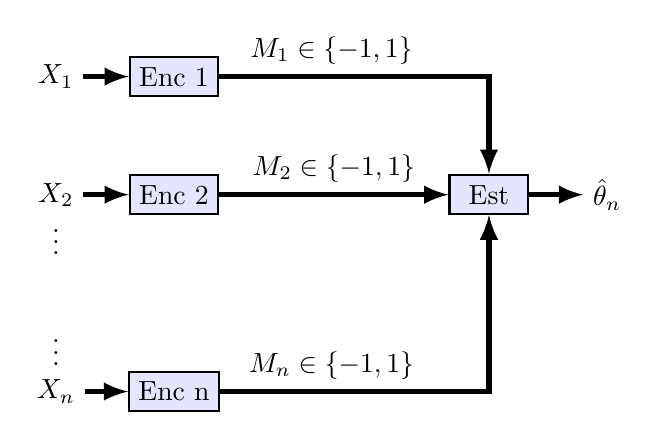
\begin{tikzpicture}[node distance=2cm,auto,>=latex]
  \node at (0,0) (source) {$X_1$} ;
  \node[int1, right of = source, node distance = 1.5cm] (enc1) {Enc 1};  
\draw[->,line width = 2pt] (source) -- (enc1); 

 \node[below of = source, node distance = 1.5cm] (source2) {$X_2$};
\node[int1, right of = source2, node distance = 1.5cm] (enc2) {Enc 2};  
\draw[->,line width = 2pt] (source2) -- (enc2); 

\node[below of = source2, node distance = 2.5cm] (source3) {$X_n$};
\node[int1, right of = source3, node distance = 1.5cm] (enc3) {Enc n};  
\draw[->,line width = 2pt] (source3) -- (enc3); 

%\node[above of = source3, node distance = 1cm] (dist) {$X_i \sim {\mathcal N} \left(\theta, \sigma^2 \right)$};
\node[below of = source2, node distance = 0.5cm] {$\vdots$};
\node[above of = source3, node distance = 0.6cm] {$\vdots$};

\node[int1, right of = enc2, node distance = 4cm ] (est) {Est};
\draw[->,line width = 2pt] (enc1) -| node[above, xshift = -2cm] (mes1) {$M_1 \in \left\{-1,1\right\}$} (est);   

\draw[->,line width = 2pt] (enc2) -- node[above, xshift = 0cm] (mes2) {$M_2 \in \left\{-1,1\right\}$} (est);   

\draw[->,line width = 2pt] (enc3) -| (est);   

\draw[->,line width = 2pt] (enc3) -| node[above, xshift = -2cm]  {$M_n \in \left\{-1,1\right\}$} (est);   

\node[right of = est, node distance = 1.5cm] (dest) {$\hat{\theta}_n$};
%         \node [int1] (dec) [right of=dest, node distance = 1.5cm,  align=center] {\small Dec };
%\node [int1] (enc) [right of = dec, node distance = 3cm]{Enc}; 
%\draw[->,line width=2pt] (dec) -- (dest);
\draw[->, line width=2pt] (est) -- (dest);
\end{tikzpicture}
\end{center}
\caption{\label{fig:distributed} Distributed one-bit encoding: the one-bit message produced by each encoder is only a function of its private sample $X_i$.}
\end{figure}
Let $f(x)$ be a symmetric and log-concave density function with a finite second moment $\sigma^2$. For $\theta \in \Theta$, denote by $P_X$ the probability distribution with density $f\left( x-\theta \right)$. Therefore, $P_X$ is an absolutely continuous log-concave distribution with mean $\theta$ and variance $\sigma^2$. Symmetry and log-concavity of $f(x)$ imply that $P_X$ is strongly unimodal with its mode at $x =\theta$ \cite{ibragimov1956composition}. We further assume that the \emph{parameter space} $\Theta$ is a closed interval of the real line. 
\par
In some situations it is useful to assume that $\theta$ is drawn once from the prior distribution $\pi$ on $\Theta$. In this case we assume that $\pi$ is an absolutely continuous distribution, and denote its density by $\pi(\theta)$, i.e., $\pi(d\theta) = \pi(\theta)d\theta$.  
\par
The random variables $X_1,\ldots,X_n$ represent $n$ independent samples from $P_X$. 
We are interested in estimating $\theta$ from a set of $n$ binary messages $M_1,\ldots,M_n$, obtained from $X_1,\ldots,X_n$ under three possible scenarios: 
\begin{itemize}
\item[(i)~~] Centralized $M_i(X_1,\ldots,X_n)$, $i=1,\ldots,n$ (Fig.~\ref{fig:centralized}).
\item[(ii)~] Adaptive $M_i(X_i,M_1,\ldots,M_{i-1})$, $i=2,\ldots,n$ (Fig.~\ref{fig:sequential}).
\item[(iii)] Distributed $M_i(X_i)$, $i=1,\ldots,n$ (Fig.~\ref{fig:distributed}).
\end{itemize}

The performance of an estimator $\hat{\theta}_n \triangleq \hat{\theta}_n(M^n)$ in any of these cases is measured according to the mean squared error (MSE) risk:
\begin{equation}
\label{eq:error_def}
R_n \triangleq \mathbb E\left(\hat{\theta}_n - \theta \right)^2,
\end{equation}
where the expectation is taken with respect to the distribution of $X^n$ and, whenever available, a prior distribution $\pi(\theta)$ over $\Theta$.  
%It is well known that minmax estimation error 
%\begin{equation}
%R_n = \min \sup_{\theta \in \Theta}  \mathbb E\left[ \left(\hat{\theta}_n - \theta \right)^2 | \theta \right],
%\end{equation}
%can be obtained from $R_n$ by assuming a particular least favorable prior distribution on the parameter space $\Theta$ \cite{casella1981}. 
%
The main problems we consider in this paper are the minimal value of \eqref{eq:error_def}, as a function of $n$ and $f(x)$, under different choices of the encoding functions in cases (i), (ii), and (iii). \\

We give particular attention to the ARE of estimators with respect to an asymptotically normal efficient estimator that is not subject to the bit constraint. Specifically, let $\{a_n,\,n\in \mathbb N\}$ be a sequence such that 
\[
\sqrt{a_n}\left(\hat{\theta}_n - \theta\right) \overset{D}{\longrightarrow} \mathcal N(0, \sigma^2).
\]
Then the ARE of $\hat{\theta}_n$ with respect to an unconstrained efficient estimator for $\theta$ is defined as \cite[Def. 6.6.6]{lehmann2006theory}
\[
\ARE(\hat{\theta}_n) \triangleq
\lim_{n\rightarrow \infty} \frac{a_n}{n}. 
\]
Note that in the special case where there exists $V \in \mathbb R$ such that
\[
a_n \mathbb E \left(\hat{\theta}_n - \theta \right)^2 = V + o(1),
\]
with $o(1)\to 0$ as $n\to \infty$, then the ARE of $\hat{\theta}_n$ is finite and equals $\sigma^2/V$. \\

In addition to the notation above, we also denote by $F(x)$ the cumulative distribution function of $X_i$, and define
\begin{equation} \label{eq:eta_def}
\eta(x) \triangleq \frac{f^2(x)}{F(x)(1-F(x))} =  \frac{f(x)f(-x)}{F(x)F(-x)}, 
\end{equation}
where the last equality is due to symmetry of $f(x)$. We note that 
\begin{equation}
\label{eq:eta_h}
\eta(x) = h(x)h(-x) = f(x) \left( h(x) + h(-x) \right), 
\end{equation}
where 
\[
h(x) \triangleq \frac{f(x)}{1-F(x)} = \frac{f(x)}{F(-x)}
\]
is the \emph{hazard} function (a.k.a. \emph{failure rate} or \emph{force of mortality}), which is a monotone increasing function since $f(x)$ is log-concave \cite{bagnoli2005log}. 
%
For $f(x)$ the normal density, it is shown in \cite{Samford1953} and \cite{hammersley1950estimating} that $\eta(x)$ is a strictly decreasing function of $|x|$, as illustrated in Fig.~\ref{fig:eta}. 
%
In this paper we only consider the normal distribution and other log-concave symmetric distributions for which this property of $\eta(x)$ holds. Specifically, we require the following:
\begin{assump} \label{assump:failure_rate}
 $\eta(x)$ is strongly unimodal. 
\end{assump}
%That is, Assumption~\ref{assump:failure_rate} says that $\eta'(x) < 0 $ for all $x>0$. 
Under this assumption we have, 
\[
4f^2(x) \leq \eta(x) \leq \eta(0),
\] 
%
where $\eta(0) = 4 f^2(0)$ is the asymptotic variance of the sample median. Combined with log-concavity of $f(x)$, Assumption~\ref{assump:failure_rate} implies that $\eta(x)$ vanishes as $|x|\rightarrow \infty$. \par
%
Assumption~\ref{assump:failure_rate} is satisfied, for example, by the generalized normal distributions with a shape parameter between $1$ and $2$ (including normal and Laplace distributions). Symmetric log-concave distributions that do not satisfy Assumption~\ref{assump:failure_rate} include the uniform distribution and the generalized normal distribution with shape parameter greater than $2$.
\\

\begin{figure}
\begin{center}
\begin{tikzpicture}[scale = 0.6]
\begin{axis}[
width=8cm, height=6cm,
xmin = -3, xmax=3, 
restrict y to domain = 0:100,
ymin = 0,
ymax = 0.9,
samples=10, 
xlabel= $x$,
xtick={-2,-1,0,1,2},
xticklabels={-2,-1,0,1,2},
ytick={0,0.3989423,0.6366198},
yticklabels={0,$\frac{1}{\sqrt{2 \pi}}$,$2/\pi$},
line width=1.0pt,
mark size=1.5pt,
ymajorgrids,
xmajorgrids,
legend style= {at={(1,1)},anchor=north east,draw=black,fill=white,align=left}
]
\addplot[color = blue, solid, smooth] plot table [x = x, y = y, col sep=comma] {./Figs/eta.csv};
\addlegendentry{$\eta(x)$};
\addplot[domain = -5:5, samples = 50, color = red, solid, smooth]  {exp(-x^2/2) / sqrt(2*3.14159)};
\addlegendentry{$\phi(x)$};
\addplot[domain = -5:5, samples = 50, color = black, solid, dashed]  {4*exp(-x^2) / (2*3.14159)};
\addlegendentry{$4\phi^2(x)$};

\end{axis}
\end{tikzpicture}
%
\begin{tikzpicture}[scale = 0.6]
\begin{axis}[
width=8cm, height=6cm,
xmin = -4, xmax=4, 
restrict y to domain = -10:0,
ymin = -10,
samples=10, 
xlabel= $x$,
xtick={-3,-2,-1,0,1,2,3},
xticklabels={-3,-2,-1,0,1,2,3},
ytick={0,-0.45158,-0.919},
yticklabels={0,,},
line width=1.0pt,
mark size=1.5pt,
ymajorgrids,
xmajorgrids,
legend style= {at={(1,1)},anchor=north east,draw=black,fill=white,align=left}
]
\addplot[color = blue, solid, smooth] plot table [x = x, y = logy, col sep=comma] {./Figs/eta.csv};
\addlegendentry{$\log \eta(x)$};
\addplot[domain = -5:5, samples = 30, color = red, solid, smooth]  {-(x)^2/2 -0.9189};
\addlegendentry{$\log \phi(x)$};
\end{axis}
\end{tikzpicture}
\caption{
The function $\eta(x) = f^2(x) / F(x)F(-x)$ for $f(x) = \phi(x)$ the standard normal density.
\label{fig:eta}
}
\end{center}
\end{figure}

\section{ Consisten Estimation and Of-the-shelf Bounds \label{sec:preliminary}}
On a first impression, it may not be clear whether consistent estimation of the mean is even possible in the adaptive and centralized settings. On the other hand, it may seem as if estimation in these cases is trivial as in the centralized setting (i). 
%
We next settle such skepticism by deriving lower and upper bounds to the relative efficiency under setting (iii). We show that:
\begin{itemize}
\item[I.] A consistent estimator with an asymptotically normal distribution always exists in setting (iii), and hence in setting (ii). 
\item[II.] For the normal distribution, the ARE in setting (iii) is at most $3/4$. Namely, under setting (iii), all estimators are strictly inferior compared to the sample mean. 
\end{itemize}

\subsection{Consistent Estimation}
Fix $\theta_0 \in \mathbb R$ and define the $i$th message by 
\[
M_i = \mathbf 1_{X_i>\theta_0}, 
\]
where $\mathbf 1_A$ is the indicator of the event $A$. We have
\[
p_n \triangleq\frac{1}{n} \sum_{i=1}^n M_i \overset{a.s.}{\rightarrow} F(\theta - \theta_0),  
\]
so that 
\begin{equation}
\label{eq:estimator_naive}
\hat{\theta}_n = \theta_0 + F^{-1}\left( p_n \right)
\end{equation}
is a consistent estimator for $\theta$ in the distributed setting of Fig.~\ref{fig:distributed}, where we note that $F(x)$ is invertible over the support of $f(x)$ which is a connected set. Furthermore, the variance of $p_n$ is $F(\theta-\theta_0)F(\theta_0-\theta)$, and hence the delta method implies that $\hat{\theta}_n$ is asymptotically normal with variance 
\begin{equation} 
\frac{1}{
\eta(\theta-\theta_0)} = \frac{F(\theta-\theta_0)F(\theta_0-\theta)}{f^2(\theta-\theta_0)}. 
\end{equation}
In particular, the ARE of $\hat{\theta}_n$ equals $\eta(\theta - \theta_0)\sigma^2$. In other words, for a prescribed accuracy, $\hat{\theta}_n$ of  \eqref{eq:estimator_naive} estimates $\theta$ with sample size that is $\eta(\theta- \theta_0)  \sigma^2$ times the samples size required for the sample mean. \par
%
%
Assumption~\ref{assump:failure_rate} implies that for  all $n$ large enough the ARE of $\hat{\theta}_n$ of \eqref{eq:estimator_naive} is never greater than $\eta(0)$, which is the ARE of the sample median. This ARE is attained only when $\theta_0 = \theta$, although $\theta$ is unknown apriori. Since $\eta(x)$ vanishes as $|x|\rightarrow \infty$, the ARE of $\hat{\theta}_n$ may be very small when $\theta$ is away from $\theta_0$. As an example, when $f(x)$ is a normal density, the ARE of $\hat{\theta}_n$ is $\approx 0.07$ when $\theta_0$ is $2.33$ standard deviations from $\theta$. Therefore, the estimator $\hat{\theta}_n$ has little practical value unless the radius of $\Theta$ is small compared to the standard deviation. \par 
It is suggested that lower variance can be obtained by an estimator of the form \eqref{eq:estimator_naive} if, after observing a batch of the single bit messages, one can update the threshold value $\theta_0$. Such a scheme falls within the adaptive setting of Fig.~\ref{fig:sequential} which we consider in Section~\ref{sec:sequential}. \\
% variance equals to $1/\eta(0)n + o(1)$. We also show in Section~\ref{sec:sequential} that no estimator can attain variance that is asymptotically smaller than $1/\eta(0)n$, so that the ARE of any estimator in settings (ii) and (iii) is at least $\eta(0) \sigma^2$. 

\subsection{Multiterminal Source Coding \label{sec:ceo}}
The CEO setting considers the estimation of a sequence $\theta_1,\theta_2\ldots$, where a noisy version of each $\theta_i$ is available at $n$ terminals. At each terminal $i$, an encoder observes the $k$ noisy samples
\[
X_{i,j} = \theta_j + Z_{i,j},\qquad j=1,\ldots,k, \qquad i = 1,\ldots,n,
\]
and transmits $R_i k$ bits to a central estimator  \cite{berger1996ceo}.  \par
%
Assuming that $\theta$ is drawn once from the prior $\pi(d\theta)$, our mean estimation problem from one-bit samples under distributed encoding in Fig.~\ref{fig:distributed} corresponds to the CEO setting with $k=1$ realization of $\theta$ observed under noise at $n$ different locations, and communicated at each location using an encoder sending a single bit. As a result, a lower bound on the MSE in estimating $\theta$ in the distributed encoding setting is given by the minimal MSE in the CEO setting as $k \to \infty$. Note that the difference between the CEO setting and ours lays in the privilege of each of the encoders to describe $k$ realizations of $\theta$ using $k$ bits with MSE averaged over these realizations, rather than a single realization using a single bit in ours. 
 \par
An optimal scheme for the CEO and its corresponding MSE is known only for the case where the prior on $\theta$, as well as the noise corrupting it at each location, are Gaussian. Namely, the Gaussian CEO is obtained from our setting when the $i$th encoder uses $R_i=1$ bits to transmit a message that is a function of $X_i = \theta + \sigma Z_i$, where $Z_i$ is standard normal. Consequently, a lower bound on the MSE in our distributed setting is obtained by considering the minimal MSE in the Gaussian CEO as the number of encoders $n$ goes to infinity. This leads to the following proposition:
\begin{prop} \label{prop:ceo_lower_bound}
Assume that $\Theta = \mathbb R$ and $\pi(\theta) = \mathcal N(0,\sigma_\theta^2)$. Then any estimator $\hat{\theta}_n$ of $\theta$ in the distributed setting satisfies
\begin{equation} \label{eq:ceo_bound}
 n\mathbb E \left( \theta - \theta_n \right)^2 \geq \frac{4\sigma^2}{3} + O(n^{-1}),
\end{equation}
where the expectation is with respect to $\theta$ and $X^n$.
\end{prop}

\begin{proof}
We consider the minimal distortion $D^\star$ in the Gaussian CEO setting with $L$ observers and under a total sum-rate $R_\Sigma = R_1 + \ldots +R_L$
from \cite[Eq. 10]{chen2004upper}:
\begin{equation} \label{eq:ceo_optimal_sumrate}
R_{\Sigma} = \frac{1}{2} \log^+ \left[ \frac{\sigma_\theta^2}{D^\star} \left( \frac{D^\star L}{ D^\star L - \sigma^2 + D^\star \sigma^2 / \sigma_\theta^2 }\right)^L  \right].
\end{equation}
For the special case of $R_\Sigma = n$ and $L=n$, we get
\begin{equation} \label{eq:ceo_optimal_sumrate2}
n = \frac{1}{2} \log_2 \left[ \frac{\sigma_\theta^2}{D^\star} \left(\frac{ D^\star n }{D^\star n - \sigma^2 + D^\star \sigma^2/\sigma_\theta^2 }  \right)^n  \right].
\end{equation}
$D^\star$ satisfying \eqref{eq:ceo_optimal_sumrate2} describing the MSE under an optimal allocation of the sum-rate $R_\Sigma = n$ among the $n$ encoders. Therefore, this $D^\star$ provides a lower bound to the CEO distortion with $R_1=\ldots,R_n = 1$ and hence a lower bound to the minimal MSE in estimating $\theta$ in the distributed setting of Fig.~\ref{fig:distributed}. By considering $D^\star$ in \eqref{eq:ceo_optimal_sumrate2} as $n\rightarrow \infty$, we see that 
\[
D^\star = \frac{ 4\sigma^2 }{3n + 4 \sigma^2 / \sigma_\theta^2 } + o(n^{-1}) =  \frac{4\sigma^2}{3n} + o(n^{-1}). 
\]
\end{proof}
We note that although the lower bound \eqref{eq:ceo_bound} was derived assuming the optimal allocation of $n$ bits per observation among the encoders, this bound cannot be tightened by considering the CEO distortion while enforcing the condition $R_1=\ldots = R_n = 1$. Indeed, an upper bound for the CEO distortion under the condition $R_1=\ldots = R_n = 1$ follows from \cite{KipnisRini2017}, and leads to
\[
D^\star \leq  \left( \frac{1}{\sigma_\theta^2} +  \frac{3n}{4\sigma^2 + \sigma_\theta^2} \right)^{-1}   =
\frac{4 \sigma^2}{3n} +  \frac{\sigma_\theta^2}{3n} + O(n^{-2}),
\]
which is equivalent to \eqref{eq:ceo_bound} when $\sigma_\theta$ is small. \par
From the formulation of the CEO problem, it follows that the difference between the MSE lower bound \eqref{eq:ceo_bound} and the actual MSE in the distributed setting (case (iii)) is exclusively attributed  to the ability to perform coding over blocks. Namely, each CEO encoder may encode an arbitrary number of $k$ independent realizations of $\theta$ using $k$ bits, versus only one realization with one bit in ours. In other words, it is the ability to exploit the geometry of a high-dimensional product probability space that 
distinguishes between the CEO problem with one bit per encoder and the mean estimation problem from one-bit measurements in the distributed setting of Fig.~\ref{fig:distributed}. 

\section{Adaptive Estimation \label{sec:sequential}}
The first main results of this paper, as described in Theorem~\ref{thm:adpative_lower_bound} below, states that the ARE of any adaptive estimator cannot be larger than $\eta(0)\sigma^2$, which is the ARE of the median of the sample $X_1,\ldots,X_n$. Next, we provide a particular adaptive estimation scheme that attains this maximal efficiency. Finally, in Theorem~\ref{thm:opt_one_step}, we provide an adaptive estimation scheme that is one-step optimal in the sense that at each step $i$, the chosen message $M_i$  minimizes the MSE given $X_i$ and the previous $i-1$ messages. %Numerical simulations for the case of $f(x)$ the normal density function shows that the ARE of the estimator described by this scheme is $\eta(0)\sigma^2$. 

\subsection{Maximal efficiency in adaptive setting}
Our first result asserts that the ARE of any adaptive encoding and estimation scheme is bounded from above by $\eta(0)\sigma^2$. %This result follows from the following theorem:
\begin{thm}[maximal relative effeciency] \label{thm:adpative_lower_bound}
Let $\hat{\theta}_n$ be any estimator of $\theta$ in the adaptive setting of Fig.~\ref{fig:sequential}. Assumes that $\pi(\theta)$ converges to zero at the endpoints of the interval $\Theta$. Then
\[
n\mathbb E\left[ (\theta-\hat{\theta}_n)^2 \right] \geq   \frac{n}{ 4f^2(0) n + I_0},
\]
where 
\[
I_0 = \mathbb E \left( \frac{d}{d\theta} \log \pi (\theta) \right)^2
\]
is the Fisher information with respect to a location model in $\theta$. 
\end{thm}

\subsubsection*{Sketch of Proof}
The main idea in the proof is to bound from above the Fisher information of any set of $n$ one-bit messages with respect to $\theta$. Once this bound is achieved, the result follows by using the van-Trees inequality \cite[Thm. 2.13]{tsybakov2008introduction},\cite{gill1995applications} which bounds from below the MSE of any estimator of $\theta$ by the inverse of the expected value of the aforementioned Fisher information plus $I_0$. The details are in the Appendix.\\

Theorem~\ref{thm:adpative_lower_bound} implies that any estimator $\hat{\theta}_n$ from any adaptive encoding scheme satisfies
\[
n\mathbb E\left[ (\theta-\theta_n)^2 \right] \leq  \frac{1}{4f^2(0)}+O(n^{-1}),
\]
and 
\[
\ARE(\hat{\theta}_n) \leq 4f^2(0)\sigma^2 = \eta(0)\sigma^2.
\]

Next, we present an adaptive encoding and estimation scheme that attains the maximal ARE of $\eta(0)\sigma^2$. 

\subsection{Asymptotically optimal estimator}
Let $\left\{ \gamma_n,\, n\in \mathbb N \right\}$ be a strictly positive sequence. Consider the following estimator $\hat{\theta}_n$ for $\theta$:  
\begin{equation}
\label{eq:sgd_alg}
\theta_n = \theta_{n-1} +  \gamma_n M_n, \quad n = 1,2,\ldots,
\end{equation}
where 
\begin{equation}
M_n = M_n (X_n,\theta_{n-1}) =\sgn (X_n - \theta_{n-1}).
\end{equation}
Define the $n$th step estimation as
\begin{equation} \label{eq:sgd_est}
\hat{\theta}_n =  \frac{1}{n} \sum_{i=1}^n  \theta_i. 
\end{equation}

We have the following results:
\begin{thm} \label{thm:sgd}
Consider the sequence $\left\{\hat{\theta}_n,\, n\in \mathbb N \right\}$ defined by \eqref{eq:sgd_est}. 
\begin{enumerate}
\item[(i)] Assume that $\left\{ \gamma_n,\, n\in \mathbb N \right\}$ satisfies
\begin{equation} \label{eq:conditions1}
\begin{cases}
\frac{\gamma_n - \gamma_{n+1}}{\gamma_n} = o(\gamma_n), &  \\
\sum_{n=1}^\infty \frac{\gamma_n^{(1+\lambda)/2}} {\sqrt{n}} < \infty, & 
\mathrm{for~some~}0< \lambda \leq 1
\end{cases}
\end{equation}
(e.g., $\gamma_n = n^{-\beta}$ for $\beta \in (0,1)$). Then
\[
\sqrt{n} \left( \hat{\theta}_n - \theta \right) \overset{d}{\rightarrow} \mathcal N \left(0,  1/\eta(0) \right).
\]
\item[(ii)] Assume that in addition to \eqref{eq:conditions1}, $\left\{ \gamma_n,\, n\in \mathbb N \right\}$ satisfies
\begin{equation} \label{eq:conditions2}
\begin{cases}
\gamma_n = o(n^{-2/3}), &  \\
\sum_{n=1}^\infty \gamma_n = \infty.  & \\
\end{cases}
\end{equation}
(e.g., $\gamma_n = n^{-\beta}$ with $2/3<\beta<1$). Then
\[
\lim_{n\rightarrow \infty} n\mathbb E \left[ \left(\theta-\hat{\theta}_n \right)^2 \right] = \frac{1}{\eta(0)}. 
\]
\end{enumerate}
\end{thm}

\subsubsection*{Proof}
The asymptotic behavior of \eqref{eq:sgd_est} follows from \cite[Thm. 4]{polyak1992acceleration} and \cite[Thm. 2]{polyak1990new}. The details are in the Appendix. \\

Theorem~\ref{thm:sgd} implies that the estimator $\hat{\theta}_n$, defined by \eqref{eq:sgd_est} and \eqref{eq:sgd_alg}, attains the maximal ARE as established by Theorem~\ref{thm:adpative_lower_bound}. The update step \eqref{eq:sgd_alg} can be seen as a gradient descent step for the function $x\to |x|$ at the point $x=X_n - \theta_{n-1}$. Consequently, the procedure above is known as averaged stochastic gradient descent for minimizing $x \to |x|$ given the data $X_1,\ldots,X_n$. The minimal value of this optimization is the sample median, and Theorem~\ref{thm:sgd} provides conditions for the sequence of gradient steps so that the algorithm converges to this minimum. 
 \par
%Note that $\theta_0$ is not explicitly defined in equation \eqref{eq:sgd_est}. A reasonable initialization for $\theta_0$ is $\theta_0 = \mathbb E [\theta]$, although Theorem~\ref{thm:sgd} implies that the asymptotic behavior of the estimator is indifferent to this initialization. Thus, the optimal efficiency is attained regardless of the prior distribution on $\theta$ or the radius of the parameter space $\Theta$.  \\
In the encoding and estimating procedure \eqref{eq:sgd_alg} and \eqref{eq:sgd_est}, each one-bit message $M_n$ is a function of the current gradient descent estimate $\theta_{n-1}$ and its private sample. As we explain next, it is possible to obtain the optimal efficiency of $\eta(0)\sigma^2$ using only a single ``access'' to such state.  

\subsection{Optimality using a Single Interaction}
In Section~\ref{sec:preliminary} we considered an estimator that is based on messages of the form 
\[
M_i = \mathbf 1_{X_i > \theta_0},\qquad i=1,\ldots,n,
\]
and showed that it is asymptotically normal with variance $1/\eta(\theta-\theta_0)$.
%
We now show that a similar encoding leads to an asymptotically normal estimator with the minimal variance $1/\eta(0)$, provided we may update once the threshold value $\theta_0$. In this procedure we separate the sample into two disjoint sets: $X_1,\ldots,X_{n_1}$ and $X_{n_1+1},\ldots,X_n$ for some $n_1 < n$. We first use the estimator \eqref{eq:estimator_naive} to obtain an estimate $\hat{\theta}_{n_1}$ based on $M_1,\ldots,M_{n_1}$, and then use $\hat{\theta}_{n_1}$ as the new threshold value to obtain messages $M_{n_1+1}, \ldots, M_n$. The specific encoding and estimation scheme, as well as its asymptotic performance, are given by the following theorem:
\begin{thm}
For $i=1,\ldots,n$ set
\[
M_i = \begin{cases}
 \mathbf 1_{X_i \geq \theta_0} & i = 1,\ldots,n_1, \\
 \mathbf 1_{X_i \geq \hat{\theta}_{n_1} }& i={n_1+1,\ldots,n},
\end{cases}
\]
where $n = n_1+ n_2$ and 
\[
\hat{\theta}_{n_1} \triangleq \theta_0 + F^{-1}\left(
\frac{1}{n_1} \sum_{i=1}^{n_1} M_i 
 \right).
\] 
Let 
\[
\hat{\theta}_{n_2}  = \hat{\theta}_{n_1} +  F^{-1} \left( \frac{1}{n_2} \sum_{i=n_1+1}^{n_2} M_i \right)
\]
and assume that $n_1(n) \rightarrow \infty$ and $n_1(n)/n \rightarrow 0$. Then:
\begin{align*}
 \sqrt{n} \left( \hat{\theta}_{n_2} - \theta  \right)^2  \overset{D}{\longrightarrow}  \mathcal N\left( 0, 1/\eta(0) \right).
\end{align*}
\end{thm}
%
%
\begin{proof}
For $t\in \mathbb R$, set
\[
p_{n_2}(t) \triangleq \frac{1}{n_2} \sum_{i=n_1+1}^{n} \mathbf 1_{X_i \geq t}. 
\]
From the central limit theorem
\begin{align*}
& \sqrt{n} \left( p_{n_2}(t) - F( \theta - t) \right)  = \sqrt{\frac{n}{n_2}} \sqrt{n_2} \left(  p_{n_2}(t) - F(\theta - t) \right) \\
& \overset{D}{\rightarrow} \mathcal N\left( 0, V(t) \right),
\end{align*}
where
\[
V(t) \triangleq F(\theta - t) F \left( t - \theta\right). 
\]
Applying the delta method to $p_{n_2}(t)$ with $g(x) = F^{-1}(x)$ we obtain
\begin{align*}
& \sqrt{n} \left( t + F^{-1}(\hat{p}_{n_2}(t)) - \theta \right) \\
&= \sqrt{n} \left( g(\hat{p}_{n_2}(t)) - g \left(F(\theta-t) \right)  \right) \\
& \overset{D}{\to} \mathcal N\left(0, 
1/\eta(\theta-t) \right).
\end{align*}
%where this convergence is uniform in $t$ since all moments of $F^{-1}(\hat{p}_{n_2})$ exists. 
By the law of large numbers we also have
\[
p_{n_1} \triangleq \frac{1}{n_1} \sum_{i=1}^{n_1} M_i \overset{a.s.}{\rightarrow} F(\theta - \theta_0),
\]
so that $\hat{\theta}_{n_1}$ converges almost surely to $\theta$ as $n$ goes to infinity, and thus 
\[
\eta( \hat{\theta}_{n_1}-\theta) \overset{a.s.}{\rightarrow} \eta(0). 
\]
By Slutsky's theorem we get
\begin{align*}
& \sqrt{n}\left(\hat{\theta}_{n_2} - \theta\right) \\
& = \sqrt{n} \left( \hat{\theta}_{n_1} + F^{-1}(\hat{p}_{n_2}(\hat{\theta}_{n_1})) - \theta \right)  \\
& \overset{D}{\to} \mathcal N\left( 0, 
1/\eta(0) \right). 
\end{align*}
\end{proof}
%

To conclude the adaptive estimation setting, we now consider estimation from one-bit messages obtained via an encoding scheme that is one-step optimal. %Namely, each message obtained by employing the optimal the decision rule given the prior distribution and the previous messages.

\subsection{One-step optimal estimation}
We now consider an estimation scheme that posses the property of \emph{one-step optimality}: at each step $n$, the $n$th encoder designs the detection region $M_n^{-1}(1)$ such that the MSE given $M^n$ is minimal. In other words, this scheme designs the messages in a greedy manner, such that the MSE at step $n$ is minimal given the current state of the estimation described by $M^{n-1}$. \\

The following theorem determine the message, i.e., the decision rule $(M^{n-1},X_n)\rightarrow M_n$, that minimizes the next step MSE:
\begin{thm}[optimal one-step estimation] \label{thm:opt_one_step}
Let $\pi(\theta)$ be an absolutely continuous log-concave probability distribution. Given a sample $X$ from a log-concave distribution with mean $\theta$, define 
\begin{equation}
\label{eq:adaptive_main_message}
M^\star = \sgn(X - \tau),
\end{equation}
where $\tau$ satisfies the equation
\begin{equation}
 \label{eq:fixed_point}
 \tau = \frac{m^-(\tau) + m^+(\tau)}{2},
\end{equation}
with
\begin{align*}
m^-(\tau)  & = \frac{\int_{-\infty}^{\tau} \theta \pi(d\theta) }{\int_{-\infty}^{\tau} \pi(d\theta)} ,\\
m^+(\tau) & = \frac{\int_{\tau}^\infty \theta \pi(d\theta) }{\int_{\tau}^\infty \pi(d\theta)} .
\end{align*}
For any estimator $\hat{\theta}$ which is a function of $M(X) \in \{-1,1\}$,
\begin{equation}
\label{eq:opt_cond}
\mathbb E \left(\theta-\hat{\theta}(M)\right)^2 \geq  \mathbb E \left(\theta- \mathbb E[\theta|M^\star]\right)^2.
\end{equation}
\end{thm}

\begin{proof}
The proof is the result of the following two lemmas, proofs of which can be found in the Appendix:
\begin{lem} \label{lem:unique}
Let $f(x)$ be a log-concave density function. Then the equation 
\begin{equation}
\label{eq:lem_fixed_point}
2x = \frac{\int_x^\infty uf(u)du}{\int_x^\infty f(u)du} + \frac{\int_{-\infty}^x uf(u)du}{\int_{-\infty}^x f(u)du} 
\end{equation}
has a unique solution.
\end{lem}
\begin{lem} \label{lem:adaptive}
Let $U$ be an absolutely continuous random variable with PDF $P(du)$. Set 
\[
M^\star(u)  =  \sgn(u - \tau),
\]
where $\tau$ is the unique solution to
 \[
2 \tau = \frac{\int_{\tau}^\infty u P(du)} {\int_{\tau}^\infty P(du)} + \frac{\int_{-\infty}^{\tau} u P(du)}{\int_{-\infty}^{\tau} P(du)}.
\]
Then for any measurable $M: \mathbb R\to \{-1,1\}$,
\[
\int \left( u - \mathbb E[U|M^\star (u)]  \right)^2 P(du) \leq \int \left( u - \mathbb E[U|M(u)]  \right)^2 P(du). 
\]
\end{lem}
\end{proof}

\begin{rem}
The optimal threshold given in Theorem~\ref{thm:opt_one_step} is different than the one given in \cite[Eq. 5]{1619423} for apparently the same problem. Indeed, it seems like Equation 4 in 
\cite{1619423} is erroneous. 
\end{rem}

By applying the optimal one-step decision rule from Theorem~\ref{thm:opt_one_step} at each step, we arrive at the following adaptive encoding and estimation scheme: 
\begin{itemize}
\item Initialization: set $P_0(t) = \pi(t)$ and $\tau_0 = \mathbb E \theta$. 
\item For $n\geq 1$:
\begin{enumerate}
\item[(1)] Update the prior as
\begin{align}
& P_n(t) = P(\theta=t |M^n) \nonumber \\
& \quad = \frac{ P\left( \theta=t | M^{n-1} \right) P(M_n | \theta = t , M^{n-1})  } { P(M_n | M^{n-1} )} \nonumber \\ 
& \quad = \alpha_n  P_{n-1}(t) F\left(M_n (t - \tau_{n-1}) \right), \label{eq:density_update}
\end{align}
where $\alpha_n$ is given by
\[
\alpha_n = \left(\int_{\mathbb R} P_{n-1}(t) F \left(M_n (t- \tau_{n-1}) \right)  dt \right)^{-1}. 
\]
\item[(2)] The $n$th estimate for $\theta$ is the conditional expectation of $\theta$ given $M^n$, namely
\begin{equation}
\theta_n = \mathbb E \left[ \theta| M^n\right] = \int_{-\infty}^\infty t P_n(t) dt. \label{eq:estimator_update}
\end{equation}
\item[(3)] Obtain $\tau_n$ from equation \eqref{eq:fixed_point} with the updated prior $P_n(t)$. Note that if $P_{n-1}(t)$ and $F(x)$ are log-concave, so does $P_n(t)$. Therefore, $P_n(t)$ is log-concave by induction and a unique solution to \eqref{eq:fixed_point} is guaranteed by Lemma~\ref{lem:unique}. 
\item[(4)] Update the $(n+1)$th message as
\begin{equation}\label{eq:message_update}
M_{n+1} = \sgn(X_{n+1}-\tau_n)
\end{equation}
\end{enumerate}
\end{itemize}
%Since Equation \eqref{eq:fixed_point} has no analytic solution in general, it is hard to derive the asymptotic behavior of the estimator defined by \eqref{eq:estimator_update} and \eqref{eq:message_update}. We conjecture, however, that it attains the asymptotic relative efficiency of $4f^2(0)$ under the same conditions on $f(x)$ in the problem formulation. 
The normalized MSE of the estimator defined by \eqref{eq:estimator_update} and \eqref{eq:message_update} is illustrated in Fig.~\ref{fig:adaptive_error} in the case where $f(x)$ is the standard normal density. Also shown in Fig.~\ref{fig:adaptive_error} are the normalized MSE of the asymptotically optimal estimator defined by \eqref{eq:sgd_alg} and \eqref{eq:sgd_est}, as well as the MSE achieved by the sample mean for the same sample realization. 

\begin{figure}
\begin{center}
\begin{tikzpicture}[scale = 0.6]
\begin{axis}[
width=10cm, height=6cm,
xmin = 0, xmax=800, 
restrict y to domain = 0:3,
ymin = 0,
ymax = 3.4,
samples=10, 
xlabel= $n$,
ylabel = {$n\mathbb E \left[\left(\theta - \hat{\theta}_n \right)^2 \right]$},
%xtick={-3,-2,-1,0,1,2,3},
%xticklabels={-3,-2,-1,0,1,2,3},
ytick={0,1,1.57},
yticklabels={0,1,$\pi/2$},
line width=1.0pt,
mark size=1.5pt,
ymajorgrids,
xmajorgrids,
legend style= {at={(1,1)},anchor=north east,draw=black,fill=white,align=left}
]

\addplot[color = blue, solid, smooth] plot table [x = itr, y = SGD, col sep=comma] {./SimRes/sim_res_nMonte5000.csv};
\addlegendentry{asymptotically optimal};

\addplot[color = red, solid, smooth] plot table [x = itr, y = Bayes, col sep=comma] {./SimRes/sim_res_nMonte5000.csv};
\addlegendentry{one step optimal};

\addplot[color = green!30!black, solid, smooth] plot table [x = itr, y = split, col sep=comma] {./SimRes/sim_res_nMonte5000.csv};
\addlegendentry{single interaction};

\end{axis}
\end{tikzpicture}
%\begin{tikzpicture}
%\node at (0,0) {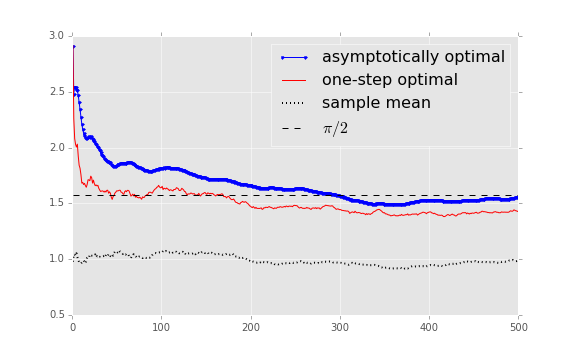
\includegraphics[scale=0.4]{one_bit_adpative}};
%\node[rotate = 90, scale = 0.7] at (-3.8,0) {$n \mathbb E \left(\hat{\theta}_n - \theta \right)^2$};
%\node[scale = 0.7] at (0,-2.4) {$n$};
%\end{tikzpicture}
\caption{Normalized empirical risk versus number of samples $n$ for $10,000$ Monte Carlo trials with $f(x)$ the standard normal density. In each trial, $\theta$ is chosen uniformly over the interval $(-1.64,1.64)$. The single interaction strategy uses $n_1 = \lfloor \sqrt{n} \rfloor$ samples for its first stage. 
\label{fig:adaptive_error}  }
\end{center}
\end{figure}


\begin{comment}
\subsection{Relation to Sigma-Delta Modulation \label{subsec:sdm}}
The SDM is a device that converts continuous-time analog signals to a discrete-time sequence of binary digits. The basic operation of a SDM can be described as follows: the modulator takes as input a sequence of continuous amplitude samples $X_n$, which are typically represents samples of a continuous-time signal taken uniformly at sampling rate $f_s$ much higher than the Nyquist rate of the signal \cite{1095151}. The output of the modulator is a sequence $M_n$ of binary values, obtained according to the following rule: 
\begin{align}
\begin{cases} V_{n+1} & =  V_n - \alpha q(V_n) + X_n, \\
M_n & = \sgn(V_n)  \end{cases}, \quad n=1,2,\ldots, \label{eq:sdm}
\end{align}
where $\alpha > 0$ is a parameter of the modulator that is determined by the maximal value of the input sequence $X^n$. The SDM of the form \eqref{eq:sdm} was studied in \cite{53738} under the assumption that the input process $X_n$ is an i.i.d Gaussian process. The main results from \cite{53738} shows that regardless of the initial state $V_0$, the process $M_n$ is a stationary ergodic process with mean $\theta$. It follows that a consistent estimation of $\theta$ is obtained by taking the mean of the sequence $\{M_n\}$. However, the results from \cite{53738} does not provide a closed form for the second order statistics of $\{M_n\}$, so that convergence rate cannot be derived from \cite{53738}.  
\end{comment}

\section{Distributed Estimation \label{sec:distributed}}
We now consider the distributed encoding setting described in Fig.~\ref{fig:distributed} (Setting (iii) in the Introduction). In this setting each one-bit message $M_i$ is only a function of its private sample $X_i$, and hence $M_i$ characterized by its \emph{detection region}, defined as 
\[
A_i = \left\{ x \in \mathbb R \,:\, M_i(x) = 1 \right\}.
\]
Consequently, $M_i$ is of the form
\[
M_i = \begin{cases} 1 & X_i \in A_i, \\
-1 & X_i \notin A_i,
\end{cases} \quad i\in \mathbb N,
\]
where the detection region $A_i$ is a Borel set that is independent of $X_1,\ldots,X_n$.\\

As a first step, we provide conditions under which the messages $M_1,M_2,\ldots$ define a local asymptotic normal family. 

\begin{thm} \label{thm:LAN1}
For $n \in \mathbb N$ and $A_n \subset \mathbb R$,  define
\begin{equation}
\label{eq:precision_general}
L_n(A_1,\ldots,A_n;\theta) \triangleq \frac{1}{n} \sum_{i=1}^n \frac{ \left(\frac{d}{d \theta} \Prob(X_i \in A_i) \right)^2 }{ \Prob(X_i \in A_i)\left(1- \Prob(X_i \in A_i) \right) }. 
\end{equation}
Consider the following conditions:
\begin{itemize}
\item [(i)\,\,] The pdf $f(x)$ of $X_n-\theta$ is a log-concave, differentiable and symmetric density function such that $\eta(x)$ is unimodal.
\item[(ii)\,] $A_n$ is a finite union of disjoint intervals.
\item[(iii)] The limit 
\begin{equation}
\label{eq:LAN_lim}
\kappa(\theta) \triangleq \lim_{n\to \infty} L_n(A_1,\ldots,A_n; \theta)
\end{equation}
exists. 
\end{itemize}
For $i=1,\ldots,n$ set
\[
M_n = \begin{cases} 1 & X_n \in A_n, \\
-1 & X_n \notin A_n. 
\end{cases} 
\]
For any $\theta$, $f(x)$ and a sequence of sets $A_1,A_2,\ldots$ such that (i)-(iii) hold, and any $h\in \mathbb R$, we have
\begin{align*}
& \log  \frac{ \mathbb P_{\theta+h/\sqrt{n}} (M_1,\ldots,M_n) }{
\mathbb P_{\theta} (M_1,\ldots,M_n)} \\
& \overset{D}{\longrightarrow} \mathcal N\left(-\frac{1}{2} h^2 \kappa(\theta), h^2 \kappa(\theta) \right).
\end{align*} 
\end{thm}
Theorem~\ref{thm:LAN1} provides conditions under which $M_1,\ldots,M_n$ defines a LAN family with a precision parameter given by the limit in \eqref{eq:LAN_lim}. An important conclusion of this theorem follows from the local asymptotic minimax property of estimators in LAN models (e.g. \cite{van2000asymptotic}):
\begin{cor} \label{cor:LA_minimax}
Let $\hat{\theta}_n$ be an estimator of $\theta \in \Theta$ from $M_1,\ldots,M_n$ with detection regions $A_1,\ldots,A_n$. Assume that as $n$ goes to infinity, conditions (i)-(iii) of Theorem~\ref{thm:LAN1} hold. Then for any bounded, symmetric, and quasi-convex function $L$, 
\[
\liminf_{c \to \infty} \liminf_{n \to \infty} \sup_{\tau\,:\,|\theta-\tau| \leq \frac{c}{\sqrt{n} }}  \mathbb E \left[ L\left( \sqrt{n}(\hat{\theta}_{n} - \tau) \right) \right] \geq \mathbb E \left[ L (Z/\sqrt{\kappa(\theta)}) \right],
\]
where $Z \sim \mathcal N(0,1)$. In particular, for $L(x) = x^2$, 
\[
\liminf_{c \to \infty} \liminf_{n \to \infty} \sup_{\tau\,:\,|\theta-\tau| \leq \frac{c}{\sqrt{n} }}  n \mathbb E  \left( \hat{\theta}_{n} - \tau \right)^2 \geq 1/\kappa(\theta).
\]
\end{cor}
%
Corollary~\ref{cor:LA_minimax} says that when the messages define a LAN model, no estimator can attain MSE smaller than $1/\kappa(\theta)n + O(1/n)$ where $\kappa(\theta)$ is the precision parameter of the model at $\theta$. This fact poses the upper bound of $\kappa(\theta)\sigma^2$ for the ARE of estimators in such models. \\

Next, we show that under LAN no estimator can attain the optimal ARE of $\eta(0)\sigma^2$ uniformly for all $\theta \in \Theta$.

\subsection{Non-existence of a Uniformly Optimal Strategy}
We now show that under LAN models, the optimal minimal risk $1/\eta(0)$ can only be attained at a finite number of points within $\Theta$. This fact implies in particular that, unlike in the adaptive setting, no distributed estimation scheme has ARE of $\eta(0)\sigma^2$ for all $\theta \in \Theta$. 

\begin{thm} \label{thm:non_existence}
Under conditions (i)-(iii) in Theorem~\ref{thm:LAN1}, assume that each $A_i$ is a union of at most $K$ intervals. The number of points $\theta \in \Theta$ satisfying $\kappa(\theta) = \eta(0)$ is at most $2K$. 
\end{thm}

\begin{proof}
See Appendix. 
\end{proof}

We next consider the case where each detection region is a half-open interval, i.e., the $i$th message is obtained by comparing $X_i$ against a single threshold. As we explain next, the existence of a density for the sequence of thresholds is enough to establish local asymptotic normality and leads to a closed form expression for the precision parameter and the ARE.  

%In the adaptive setting, it follows from Theorem~\ref{thm:sgd} that messages of this kind with appropriately chosen thresholds lead to an estimator with the optimal ARE of $\eta(0)sigma^2$. However, Theorem~\ref{thm:non_existence} implies that such ARE can only be attained for a negligible subset of the parameter space. As we shall see next, messages obtained via a comparison against a sequence of thresholds cannot attain the optimal efficiency one more than a single point of $\Theta$. 

\subsection{Threshold Detection}
Assume now that each $M_i$ is of the form
\begin{equation}
\label{eq:threshold_message}
M_i = \sgn(t_i - X_i) = \begin{cases} 1 & X_i< t_i, \\
-1 & X_i > t_i,
\end{cases}  
\end{equation}
where $t_i\in\mathbb R$ is the \emph{threshold} of the $i$th encoder. In other words, the detection region of $M_i$ is $A_i = (t_i,\infty)$ and $\mathbb P(X_i \in A_i) = F \left( M_i(t_i-\theta) \right)$. It follows that
\begin{equation}
L_n(A_1,\ldots,A_n;\theta) = \frac{1}{n} \sum_{i=1}^n \frac{ \left(f(t_i-\theta) \right)^2 }{F\left(t_i-\theta \right) F\left(\theta - t_i \right) }  = \frac{1}{n} \sum_{i=1}^n \eta(t_i - \theta).
\label{eq:Ln_threshold}
\end{equation}
A natural condition for the existence of the limit \eqref{eq:Ln_threshold} as $n\to \infty$ is that the empirical distribution of the threshold values converges to a probability measure. Specifically, for an interval $I \subset \mathbb R$ define
\[
\lambda_n(I) = \frac{ \card \left( I \cap \{t_1,t_2,\ldots \} \right)}{n}. 
\]
Theorem~\ref{thm:LAN1} implies:
\begin{cor} \label{cor:LAN_thresh}
Let $\{t_n\}_{n=1}^\infty$ be a sequence of threshold values such that $\lambda_n$ converges (weakly) to a probability measure $\lambda(dt)$ on $\mathbb R$. Then $\left\{ M_i = \sgn(X_i - t_i) \right\}_{i=1}^n$ is a LAN family with precision parameter
\[
\kappa(\theta) = \int_{\mathbb R} \eta(t-\theta) \lambda(dt). 
\]
\end{cor}

Due to local asymptotic normality of $\{M_n\}_{n=1}^\infty$, the maximum likelihood estimator (ML) of $\theta$ from $M_1,\ldots,M_n$, denoted here by 
$\hat{\theta}^{ML}_n$, is local asymptotic minimax in the sense that 
\[
\sqrt{n} \left( \hat{\theta}^{ML}_n - \theta \right) \overset{D}{\longrightarrow} \mathcal{N} \left(0, 1/\kappa(\theta) \right). 
\]
It follows that when the density of the threshold values converges to a probability measure, the ARE of the ML estimator is $\kappa(\theta)\sigma^2$, and this ARE is maximal with respect to all local alternative estimators for $\theta$. We note that $\hat{\theta}^{ML}_n$ is given by the root of 
\begin{equation}
\label{eq:ML}
\sum_{i=1}^n M_i \frac{f \left( t_i-\theta\right) }{F \left(M_i  (t_i-\theta)\right) },  
\end{equation}
which is the derivative of the log-likelihood function. This root is unique since the log-likelihood function is concave. Furthermore, for any $n \in \mathbb R$, we have that $\hat{\theta}^{ML}_n  \in [t_{(1)}, t_{(n)}]$ where $t_{(i)}$ denotes the $i$th element of $\{t_1,t_2\ldots\}$. Therefore, if $\{t_1,t_2\ldots\}$ is bounded (for example $\{t_1,t_2\ldots\} \subset \Theta$), then 
\[
\lim_{n\to \infty} n\left(\hat{\theta}^{ML}_n - \theta \right)  = 1/\kappa(\theta), 
\] 
so that the ML estimator attains the local asymptotic MSE of Corollary~\ref{cor:LA_minimax}. \par
%
Since $\eta(x)$ attains its maximum at the origin, we conclude that
\[
\kappa(\theta) \leq \sup_{t\in \mathbb R} \eta \left( t-\theta\right) = \eta(0).
\]
This upper bound on $\kappa(\theta)$ implies that the ARE of any distributed estimator based on a sequence of threshold detectors does not exceed $\eta(0)\sigma^2$, a fact that agrees with the lower bound under adaptive estimation derived in Theorem~\ref{thm:adpative_lower_bound}. 
%
This upper bound on $\kappa(\theta)$ is attained only when $\lambda$ is the mass distribution at $\theta$. Since $\theta$ is apriori unknown, we conclude that estimation in the distributed setting using threshold detection is strictly sub-optimal compared to the adaptive setting. In other words, the ability to choose the threshold values in an adaptive manner based on previous messages strictly improves relative efficiency compared to a non-adaptive threshold selection.  \\

%We conclude that when the density of the threshold values converges to a probability measure, the ARE of the ML is $\kappa(\theta)$, and this ARE is maximal with respect to all local alternative estimators for $\theta$. 

%
We conclude this section by considering the density of the threshold values that maximizes the ARE $\kappa(\theta)$ under the worst choice of $\theta \in \Theta$.

\subsection{Minimax Threshold Density}
The distribution $\lambda(dt)$ that maximizes $\kappa(\theta)$, and thus minimizes $1/\kappa(\theta)$, over the worst choice of $\theta$ in $\Theta = [-T,T]$ is given as the solution to the following optimization problem:
\begin{align}
\label{eq:var_cvx_minimax}
\begin{split}
\mathrm{maximize} \quad &  \inf_{\theta \in [-T,T]} \int \eta(t-\theta) \lambda(dt)
\\ 
\mathrm{subject~to} 
\quad & \lambda(dt)\geq 0,\quad \int \lambda(dt) \leq 1. 
\end{split}
\end{align}
The objective function in \eqref{eq:var_cvx_minimax} is concave in $\lambda(dt)$ and hence this problem can be solved using a convex program. We denote by $\kappa^\star(T)$ the maximal value of \eqref{eq:var_cvx_minimax} and by $\lambda^\star(dt)$ the density that achieves this maximum.  
%
%By discretizing the interval $[-b,b]$ using $N_\theta$ values $\theta_1,\ldots,\theta_{N_\theta}$ and the real line using $N_\lambda$ values $\lambda_1,\ldots,\lambda_{N_\lambda}$, the discrete version of \eqref{eq:var_cvx_minimax} is the following linear program (LP) in the variables $K \in \mathbb R$ and $\lambda \in \mathbb R^{N_\lambda}$:
%\begin{align}
%\label{eq:cvx_minimax}
%\begin{split}
%\mathrm{maximize} \quad &  K \\ 
%\mathrm{subject~to} 
%\quad &  K \leq \mathbf H\lambda \\
%& \lambda \geq 0,\quad   \mathbf 1^T\lambda  \leq 1,
%\end{split}
%\end{align}
%where $\mathbf H_{i,j} = \eta(t_i - \theta_j)$, $i=1,\ldots,N_\lambda$, $j = 1,\ldots,N_\theta$. 
%\begin{rem}
%The number of variables in \eqref{eq:cvx_minimax} is $N_\lambda+1$ and number of constraints is $1 + N_\lambda + N_\theta$. Since an LP has an optimal solution at which the number of constraints for which equality holds is no smaller than the number of variables \cite{papadimitriou1998combinatorial}, there exists an optimal $\lambda$ with support over no more than $N_{\theta}$ points. Therefore, in approximating the solution of \eqref{eq:var_cvx_minimax} using 
%\eqref{eq:cvx_minimax}, it is enough to take $N_\lambda = N_\theta$.
%\end{rem} 

Figure~\ref{fig:minimax_support} illustrates an approximating to $\lambda^\star(dt)$ obtained by solving a discretized version of \eqref{eq:var_cvx_minimax} for the case when $f(x)$ is the normal density with variance $\sigma^2$. The minimal asymptotic risk $\kappa^\star(\theta)$ obtained this way is illustrated in Fig.~\ref{fig:minimax_ARE} as a function of the support size $T$. Also illustrated in these Figures is $\kappa_{\unif}$ which is the precision parameter corresponding to threshold values uniformly distribution over $\Theta = [-T,T]$, namely
\begin{align}
& \kappa_{\unif} \triangleq \min_{\theta \in [-T,T]} \frac{1}{2T}\int_{-T}^T \eta\left(t-\theta\right) dt \nonumber
 \\
& = 
\frac{1}{2T}\int_{-T}^{T} \eta\left(t\pm T\right) dt
= \frac{1}{2T}\int_{0}^{2T} \eta(t) dt  \label{eq:uniform_risk}. 
\end{align}
From Corollary~\ref{cor:LAN_thresh}, we conclude that the ARE under a uniform distribution is $\kappa_\unif \sigma^2$. \\

\begin{figure}
\begin{center}
\begin{tikzpicture}[scale = 0.55]
\begin{axis}[
width=8cm, height=6cm,
xmin = -0.5, xmax=0.5, 
restrict y to domain = 0:100,
ymin = 0,
ymax = 1,
samples=10, 
xlabel= {$dt$},
xtick={-0.5,0,0.5},
xticklabels={-$T$, 0, $T$},
title = {$\sigma/T = 1/2$},
ytick={0,0.1,1},
%ylabel = {$\lambda(dt)$},
yticklabels={0,0.1,1},
line width=1.0pt,
mark size=1.5pt,
ymajorgrids,
xmajorgrids,
legend style= {at={(1,1)},anchor=north east,draw=black,fill=white,align=left}
]
\addplot[color = blue, smooth, mark = o ] plot table [col sep=comma] {./Figs/minmax_lmd_b0.5_sig0.5.csv};

\addplot[color = black!30!green, smooth, dashed] plot table [x = x, y  = z,col sep=comma] {./Figs/minimax_th_b0.5_sig0.5.csv};

\addplot[color = red, smooth] plot table [x = x, y  = y,col sep=comma] {./Figs/minimax_th_b0.5_sig0.5.csv};

\end{axis}
\end{tikzpicture}
%
\begin{tikzpicture}[scale = 0.55]
\begin{axis}[
width=8cm, height=6cm,
xmin = -0.5, xmax=0.5, 
restrict y to domain = 0:100,
ymin = 0,
ymax = 0.6,
samples=10, 
xlabel= {$dt$},
title = {$\sigma/T = 1/5$},
xtick={-0.5,0,0.5},
xticklabels={-$T$, 0, $T$},
ytick={0,0.5},
ylabel = {$\lambda(dt)$},
yticklabels={0,0.5},
line width=1.0pt,
mark size=1.5pt,
ymajorgrids,
xmajorgrids,
legend style= {at={(1,1)},anchor=north east,draw=black,fill=white,align=left}
]
\addplot[color = blue, smooth, mark = o ] plot table [col sep=comma] {./Figs/minmax_lmd_b0.5_sig0.2.csv};

\addplot[color = black!30!green, smooth, dashed] plot table [x = x, y  = z,col sep=comma] {./Figs/minimax_th_b0.5_sig0.2.csv};

\addplot[color = red, smooth] plot table [x = x, y  = y,col sep=comma] {./Figs/minimax_th_b0.5_sig0.2.csv};

\end{axis}
\end{tikzpicture}
%
\begin{tikzpicture}[scale = 0.55]
\begin{axis}[
width=8cm, height=6cm,
xmin = -0.5, xmax=0.5, 
restrict y to domain = 0:100,
ymin = 0,
ymax = 0.3,
samples=10, 
xlabel= {$dt$},
xtick={-0.5,0,0.5},
title = {$\sigma / T = 1/10$},
xticklabels={-$T$, 0, $T$},
ytick={0,0.2},
%ylabel = {$\lambda(dt)$},
yticklabels={0,0.2},
line width=1.0pt,
mark size=1.5pt,
ymajorgrids,
xmajorgrids,
legend style= {at={(1,1)},anchor=north east,draw=black,fill=white,align=left}
]
\addplot[color = blue, smooth, mark = o ] plot table [col sep=comma] {./Figs/minmax_lmd_b0.5_sig0.1.csv};

\addplot[color = black!30!green, smooth, dashed] plot table [x = x, y  = z,col sep=comma] {./Figs/minimax_th_b0.5_sig0.1.csv};

\addplot[color = red, smooth] plot table [x = x, y  = y,col sep=comma] {./Figs/minimax_th_b0.5_sig0.1.csv};

\end{axis}
\end{tikzpicture}
%
\begin{tikzpicture}[scale = 0.55]
\begin{axis}[
width=8cm, height=6cm,
xmin = -0.5, xmax=0.5, 
restrict y to domain = 0:100,
ymin = 0,
ymax = 0.15,
samples=10, 
xlabel= {$dt$},
title = {$\sigma / T = 1/20$},
xtick={-0.5,0,0.5},
xticklabels={-$T$, 0, $T$},
ytick={0,0.1},
ylabel = {$\lambda(dt)$},
yticklabels={0,0.1},
line width=1.0pt,
mark size=1.5pt,
ymajorgrids,
xmajorgrids,
legend style= {at={(1,1)},anchor=north east,draw=black,fill=white,align=left}
]
\addplot[color = blue, smooth, mark = o ] plot table [x = x, y  = y,col sep=comma] {./Figs/minmax_lmd_b0.5_sig0.05.csv};

\addplot[color = black!30!green, smooth, dashed] plot table [x = x, y  = z,col sep=comma] {./Figs/minimax_th_b0.5_sig0.05.csv};

\addplot[color = red, smooth] plot table [x = x, y  = y,col sep=comma] {./Figs/minimax_th_b0.5_sig0.05.csv};


%\addlegendentry{$\frac{\sigma^2}{\sigma_\theta^2} = 1$};
\end{axis}
\end{tikzpicture}

\caption{\label{fig:minimax_support}
Optimal threshold density $\lambda^\star(dt)$ (blue) that maximizes the ARE for $f(x) = \mathcal N(\theta,\sigma^2)$ and $\theta \in \Theta = [-T,T]$.
%
The continuous curve (red) represents the reciprocal of the asymptotic risk for at a fixed $\theta \in \Theta$ under the optimal density, so the minimax risk is the inverse of its minimal value. The dashed curve (green) is the reciprocal of the asymptotic risk for a fixed $\theta$ under a uniform distribution of threshold values over $\Theta$, hence its minimal value is the inverse of \eqref{eq:uniform_risk}. }
\end{center}
\end{figure}


\begin{figure}
\begin{center}
\begin{tikzpicture}[scale = 1]
\begin{axis}[
width=8cm, height=6cm,
xmin = 0, xmax=2.5, 
xmode = log,
restrict y to domain = 0:100,
ymin = 0,
ymax = 1,
samples=1, 
xlabel= {$\sigma/T$},
%xtick={-0.5,0,0.5},
%xticklabels={-$$, 0, $b$},
ytick={0,0.637,1},
yticklabels={0,$2/\pi$,1},
ylabel = {$\ARE$},
line width=1.0pt,
mark size=1.5pt,
ymajorgrids,
xmajorgrids,
legend style= {at={(1,1)},anchor=north east,draw=black,fill=white,align=left}
]
\addplot[color = red, smooth, line width = 1pt] plot table [x = x, y = y, col sep=comma] {./Figs/minmax_ARE_b0.5.csv};
\addlegendentry{optimal threshold density};

\addplot[color = black!35!green, smooth, dashed, line width = 1pt] plot table [x = x, y = z, col sep=comma] {./Figs/minmax_ARE_b0.5.csv};
\addlegendentry{uniform threshold desnity};
\end{axis}
\end{tikzpicture}
\caption{\label{fig:minimax_ARE} Minimax ARE versus $\sigma/T$ for $f(x) = \mathcal N(\theta,\sigma^2)$  and $\theta \in \Theta = [-T,T]$. The dashed curve (green) is the ARE under a uniform threshold density over $\Theta$ given by $K_{\unif}\sigma^2$, where $\kappa_{\unif}$ is given by \eqref{eq:uniform_risk}. }.
\end{center}
\end{figure}


%We have seen that using threshold detection, an ARE $\eta(0)\sigma^2$ can only be attained at a single point in $\Theta$. Next, we prove that with any set of messages obtained via a distributed strategy, there exists at least one $\theta \in \Theta$ such that the estimator of $\theta$ has ARE strictly smaller than $\eta(0)\sigma^2$. 


\begin{comment}
\subsection{Asymptotic Bayes Risk}
\begin{figure}
\begin{center}
\begin{tikzpicture}[scale = 0.55]
\begin{axis}[
width=8cm, height=6cm,
xmin = -0.5, xmax=0.5, 
restrict y to domain = 0:100,
ymin = 0,
ymax = 1,
samples=10, 
xlabel= {$dt$},
xtick={-0.5,0,0.5},
xticklabels={-$b$, 0, $b$},
title = {$\sigma/\sigma_{\theta} = 1$},
ytick={0,1},
%ylabel = {$\lambda(dt)$},
yticklabels={0,1},
line width=1.0pt,
mark size=1.5pt,
ymajorgrids,
xmajorgrids,
legend style= {at={(1,1)},anchor=north east,draw=black,fill=white,align=left}
]
\addplot[color = blue, smooth, mark = o ] plot table [col sep=comma] {./Figs/unif_Bayes_lmd_b0.5_sig1.csv};
%\addlegendentry{$\frac{\sigma^2}{\sigma_\theta^2} = 1$};
\end{axis}
\end{tikzpicture}
%
\begin{tikzpicture}[scale = 0.55]
\begin{axis}[
width=8cm, height=6cm,
xmin = -0.5, xmax=0.5, 
restrict y to domain = 0:100,
ymin = 0,
ymax = 1,
samples=10, 
xlabel= {$dt$},
title = {$\sigma/\sigma_{\theta} = 2$},
xtick={-0.5,0,0.5},
xticklabels={-$b$, 0, $b$},
ytick={0,1},
ylabel = {$\lambda(dt)$},
yticklabels={0,1},
line width=1.0pt,
mark size=1.5pt,
ymajorgrids,
xmajorgrids,
legend style= {at={(1,1)},anchor=north east,draw=black,fill=white,align=left}
]
\addplot[color = blue, smooth, mark = o ] plot table [col sep=comma] {./Figs/unif_Bayes_lmd_b0.5_sig2.csv};
%\addlegendentry{$\frac{\sigma^2}{\sigma_\theta^2} = 1$};
\end{axis}
\end{tikzpicture}
%
\begin{tikzpicture}[scale = 0.55]
\begin{axis}[
width=8cm, height=6cm,
xmin = -0.5, xmax=0.5, 
restrict y to domain = 0:100,
ymin = 0,
ymax = 1,
samples=10, 
xlabel= {$dt$},
xtick={-0.5,0,0.5},
title = {$\sigma/\sigma_{\theta} = 3$},
xticklabels={-$b$, 0, $b$},
ytick={0,1},
%ylabel = {$\lambda(dt)$},
yticklabels={0,1},
line width=1.0pt,
mark size=1.5pt,
ymajorgrids,
xmajorgrids,
legend style= {at={(1,1)},anchor=north east,draw=black,fill=white,align=left}
]
\addplot[color = blue, smooth, mark = o ] plot table [col sep=comma] {./Figs/unif_Bayes_lmd_b0.5_sig3.csv};
%\addlegendentry{$\frac{\sigma^2}{\sigma_\theta^2} = 1$};
\end{axis}
\end{tikzpicture}
%
\begin{tikzpicture}[scale = 0.55]
\begin{axis}[
width=8cm, height=6cm,
xmin = -0.5, xmax=0.5, 
restrict y to domain = 0:100,
ymin = 0,
ymax = 1,
samples=10, 
xlabel= {$dt$},
title = {$\sigma/\sigma_{\theta} = 4$},
xtick={-0.5,0,0.5},
xticklabels={-$b$, 0, $b$},
ytick={0,1},
ylabel = {$\lambda(dt)$},
yticklabels={0,1},
line width=1.0pt,
mark size=1.5pt,
ymajorgrids,
xmajorgrids,
legend style= {at={(1,1)},anchor=north east,draw=black,fill=white,align=left}
]
\addplot[color = blue, smooth, mark = o ] plot table [col sep=comma] {./Figs/unif_Bayes_lmd_b0.5_sig4.csv};
%\addlegendentry{$\frac{\sigma^2}{\sigma_\theta^2} = 1$};
\end{axis}
\end{tikzpicture}

\caption{\label{fig:opt_density}
Optimal threshold density $\lambda^\star(dt)$ that minimizes the asymptotic Bayes risk \eqref{eq:cvx_average} for a uniform prior with $\sigma/\sigma_\theta=1,2,3,4$, where $\sigma_\theta^2=b^2/3$ is the variance of the prior. 
}
\end{center}
\end{figure}

 We consider now the problem of minimizing the asymptotic Bayes risk $
R_{\pi,\lambda} \triangleq \mathbb E  K^{-1}(\theta)$ over all probability measures $\lambda(dt)$ with support in $\mathbb R$. This optimization problem can be written as follows:
\begin{align}
\label{eq:cvx_average}
\begin{split}
\mathrm{minimize} \quad & R_{\pi,\lambda} =  \int \frac{\pi(d\theta)}{ \int \eta \left( t-\theta\right) \lambda(dt)}. \\ 
\mathrm{subject~to} \quad & \lambda(dt)\geq 0,\quad \int \lambda(dt) =1. 
\end{split}
\end{align}
We denote by $R^\star_{\pi}$ the minimal value of the objective function in \eqref{eq:cvx_average}. Since the function $x \rightarrow 1/x$ is convex for positive values, \eqref{eq:cvx_average} defines a convex optimization problem in $\lambda$ whose solution depends on the prior $\pi$. The solution to this problem is approximated by considering $\lambda$ and $\pi$ over a discrete set in a similar way that \eqref{eq:cvx_minimax} is obtained from \eqref{eq:var_cvx_minimax}. \par
For the case of a normal distribution ($P_X = \mathcal N(\theta, \sigma^2)$) and a uniform prior ( $\pi(d\theta) =dt/(2b)$), the optimal asymptotic threshold density obtained as the solution to \eqref{eq:cvx_average} is illustrated in Fig.~\ref{fig:opt_density}, whereas Fig.~\ref{fig:dist_bound_uniform} illustrates the corresponding Bayes risk. 
\par
\begin{figure}
\begin{center}

\begin{tikzpicture}[scale = 1]
\begin{axis}[
width=8cm, height=6cm,
xmin = 0, xmax=2, 
restrict y to domain = 0:100,
ymin = 0,
ymax = 10,
samples=1, 
xlabel= {$\sigma/\sigma_\theta$},
%xtick={-0.5,0,0.5},
%xticklabels={-$$, 0, $b$},
ytick={0,1.5708,5},
yticklabels={0,$\pi/2$,5},
ylabel = {$R_{\pi}^\star/\sigma^2$},
line width=1.0pt,
mark size=1.5pt,
ymajorgrids,
xmajorgrids,
legend style= {at={(1,1)},anchor=north east,draw=black,fill=white,align=left}
]
\addplot[color = red, smooth] plot table [x = x, y = Runif, col sep=comma] {./Figs/unif_Bayes_Risk.csv};
%\addlegendentry{$\frac{\sigma^2}{\sigma_\theta^2} = 1$};
\addplot[color = red, smooth, dashed, line width = 0.5pt] plot table [x = x, y = Rbound, col sep=comma] {./Figs/unif_Bayes_Risk.csv};
\addplot[color = black, dashed] {3.14159 / 2};
\end{axis}
\end{tikzpicture}
\caption{Asymptotic Bayes risk $R_{\pi}^\star$ in estimating the mean of a normal distribution ($P_X = \mathcal N(\theta, \sigma^2)$under an optimal threshold distribution $\lambda^\star$ for $\pi$ the uniform distribution over $\Theta = [-0.5,0.5]$. 
%
%versus $\sigma/\sigma_\theta = 2\sqrt{3}\sigma$.
The distribution $\lambda^\star$ is the minimizer of \eqref{eq:cvx_average}. It is illustrated for various cases in Fig.~\ref{fig:opt_density}. The dashed curve represents the upper bound \eqref{eq:upper_bound}. 
\label{fig:dist_bound_uniform}  }
\end{center}
\end{figure}

As can be seen in Fig.~\ref{fig:opt_density} for the case $P_X = \mathcal N(\theta ,\sigma^2)$ and a uniform $\pi$, when the radius of $\Theta$ is small compared to $\sigma$, the optimal distribution $\lambda^\star$ is a mass distribution. In this case, the ML estimator reduces to the estimator $\hat{\theta}_n$ of \eqref{eq:estimator_naive}. As the following proposition shows, the Bayes risk for this choice of $\lambda$ is maximal, and thus provides an upper bound on the Bayes risk under any $\lambda$. 
 \eqref{eq:cvx_average}. 
\begin{prop}\label{prop:upper_bound}
For any prior $\pi(d\theta)$ and $\theta_0$ in the support of $\eta(x)$ we have
\begin{equation} 
\label{eq:upper_bound}
R_\pi^\star  \leq 
 \int \frac{\pi(d\theta)}{\eta \left( \theta_0 - \theta \right)},
\end{equation}
Furthermore, assuming that $\theta_0 = \mathbb E \theta$ and that $\pi$ has a finite third moment $\sigma_\theta^3$, we have: 
\begin{equation}
\label{eq:bound_Taylor}
R^\star_\pi \leq \frac{1}{4 f^2(0)} + \left(\frac{1}{4 f^2(0)} \frac{-f''(0)}{f(0)} -1 \right) \sigma_\theta^2 + O(\sigma_\theta^3).
\end{equation}
\end{prop}
\begin{proof}
The function $x \rightarrow 1/x$ is convex for positive values, hence Jensen's inequality implies
\[
\left( \int \eta \left( t-\theta\right) \lambda(dt) \right)^{-1}  \leq \int  \frac{ \lambda(dt)}{ \eta \left( t-\theta\right)  }. 
\]
Therefore, the expected value of $\kappa^{-1}(\theta)$ satisfies
\begin{align}
\mathbb E  \frac{1}{\kappa(\theta)}  \leq \int \int \frac{\pi(d\theta) \lambda(dt) }{\eta \left( t - \theta \right)}. \label{eq:upper_bound_proof}
\end{align}
The bound \eqref{eq:upper_bound} is obtained by taking $\lambda$ to be a mass distribution at any $\theta_0$ in the support of $\eta(x)$. Finally, \eqref{eq:bound_Taylor} is obtained by expanding $1/\eta(x)$ to a third order Taylor series around zero
%\[
%1/\eta(x) = \frac{1}{4f^2(0)}  + \left(\frac{1}{4 f^2(0)} \frac{-f''(0)}{f(0)} -1 \right)  x^2 + O(x^3),
%\]
and taking its expectation with respect to $\pi$ at $x=\theta_0-\theta$. 
\end{proof}
We note that the function $1/\eta(x)$ is quasi-convex and symmetric around zero, so taking $\theta_0 = \mathbb E \theta$ minimizes the RHS of \eqref{eq:upper_bound} among all $\theta_0$ in the support of $\eta(x)$.\par
The bound \eqref{eq:upper_bound} is not trivial as long as the integral in the RHS of \eqref{eq:upper_bound} is finite, i.e., whenever the tail of $\pi(\theta)$ vanishes fast enough compared to $\eta(x)$. The expansion \eqref{eq:bound_Taylor} implies that this bound becomes tight whenever the support of the optimal distribution is a mass distribution at $\mathbb E \theta$, in which case the expected value of $\kappa^{-1}(\theta)$ approaches $1/\eta(0) = 1/4f^2(0)$. 

\begin{example} \label{ex:bound}
In the normal case $P_X = \mathcal N(\theta, \sigma^2)$, the bound in \eqref{eq:bound_Taylor} implies 
\[
\frac{R^\star_\pi}{\sigma^2}  \leq \frac{\pi}{2} + \left( \frac{\pi}{2} -1 \right) \left( \frac{ \sigma_\theta}{\sigma} \right)^2 + O \left(  \frac{\sigma_\theta} { \sigma} \right)^3. 
\]
It follows that the ARE approaches its maximal value of $2/\pi$ whenever $\sigma_\theta/\sigma$ is small. The exact value of \eqref{eq:upper_bound} in this case, as well as the Bayes ARE with the optimal threshold density $\lambda^\star$ for a uniform $\pi$, are illustrated in Fig.~\ref{fig:dist_bound_uniform}. 
%i.e., each encoder simply reports "$1$" or "$-1$" whenever $X_i$ is larger or smaller than $\theta_0$, respectively. Intuitively, an accurate estimation of $\theta$ in this case is possible only if a sufficient mix of ''$1$''s and ''$-1$''s is obtained from the sample. When $\sigma_\theta^2$ is high compared to $\simga^2$, one of the events $"1"$ or "$-1"$ becomes too rare to
\end{example}


% The following proposition implies that this bound is always tight as $\sigma / \sigma_\theta$ goes to infinity.
%\begin{prop} \label{prop:asymp}
% For any prior $\pi(\theta)$ for which
%\[
%\int \frac{\pi(d\theta)}{\eta \left(\theta \right)} < \infty,
%\]
%we have 
%\begin{align}
%\label{eq:asymp}
%\mathbb E [1/\kappa(\theta)] = \frac{\pi}{2} + \left( \frac{\pi}{2} - 1\right) \left(\frac{\sigma_\theta}{\sigma} \right)^2 + o \left(\frac{1}{\sigma} \right)^3. 
%\end{align}
%as $\sigma_\theta / \sigma \rightarrow 0$. 
%\end{prop}
%\begin{proof}
%It is enough to prove that  \eqref{eq:asymp} holds for the upper bound \eqref{eq:upper_bound}. First note that the condition in the proposition implies that all the moments of $\pi(\theta)$ exists, and in particular its second and third. The results follows by expanding the function $1/\eta(x)$ in a power series around zero as
%\[
%1/\eta(x) = \frac{\pi}{2} + \left(\frac{\pi}{2}-1 \right) x^2 + o(x^3).
%\]
%\end{proof}
\end{comment}

\section{Conclusions \label{sec:conclusions}}
We considered the MSE risk in estimating the mean of a symmetric and log-concave distribution from a sequence of bits, where each bit is obtained by encoding a single sample from this distribution. 
%
In an adaptive encoding setting, we showed that no estimator can attain asymptotic relative efficiency (ARE) larger than that of the median of the samples. We also showed that this bound is tight by presenting two adaptive encoding and estimation procedures that are as efficient as the median. 
%We further showed that the optimal MSE and ARE can be attained using only a single adaptation. Namely, a single round of communication between {\color{red} the estimator and the encoder} . 
We also characterized the one-step optimal scheme in this adaptive setting, i.e., the scheme that minimizes the risk given any set of previously obtained bits. %Numerical simulations show that the one-step optimal scheme attains the optimal relative efficiency for the normal distribution. 
\par
In the distributed setting we provided conditions for local asymptotic normality of the encoded samples, which implies asymptotic minimax bound on both the risk and ARE. 
%
We conclude that under such conditions, the optimal estimation performance derived for the adaptive case can only be attained over a finite number of points, i.e., no scheme is uniformly optimal in the distributed setting. 
%
We further considered the special case of messages obtained by comparing against a prescribed sequence of thresholds. We characterized the performance of the optimal estimator from such messages using the density of these thresholds, and consider the threshold density that minimizes the minimax risk.
 \\


%\section*{ACKNOWLEDGMENT}
%This research is supported in parts by...
%Tsachy Weissman, Stefano Rini, Robert Gray.


\onecolumn 

\appendices

\section{Proofs \label{app:proofs}}

\begin{lem} \label{lem:bound_intervals}
Let $f(x)$ be a log-concave, symmetric, and differentiable density such that $\eta(x)$ is strongly unimodal. For any $x_1 > \ldots > x_n \in \mathbb R$, 
\begin{equation}
\frac{ \left(  \sum_{k=1}^n (-1)^{k+1} f(x_k) \right)^2} 
{\left( \sum_{k=1}^n (-1)^{k+1} F(x_k) \right)\left(1- \sum_{k=1}^n (-1)^{k+1} F(x_k) \right) } 
\leq \max_i \eta(x_i). \label{eq:lem_bound_intervals}
\end{equation}
In particular, if $|x_i|>\epsilon > 0$ for all $i=1,\ldots,n$, then 
\[
\frac{ \left(  \sum_{k=1}^n (-1)^{k+1} f(x_k) \right)^2} 
{\left( \sum_{k=1}^n (-1)^{k+1} F(x_k) \right)\left(1- \sum_{k=1}^n (-1)^{k+1} F(x_k) \right) } 
\leq \eta(\epsilon) < 0. 
\]
\end{lem}

\subsubsection*{Proof of Lemma~\ref{lem:bound_intervals}} 
Denote 
\[
\delta_n \triangleq \delta_n(x_1,\ldots,x_n) \triangleq \sum_{k=1}^{n} (-1)^{k+1} f(x_k),
\]
\[
\Delta_n \triangleq \Delta_n(x_1,\ldots,x_n) \triangleq  \sum_{k=1}^n (-1)^{k+1} F(x_k),
\]
so 
\[
\eta(x) =  \frac{  \left(\delta_1(x) \right)^2}{\Delta_1(x)
(1-\Delta_1(x))}
= \frac{  \left( f (x) \right)^2}{ F(x)\left(1-F(x)\right)^2}. 
\]
We use induction on $n \in \mathbb N$ to show that the LHS of \eqref{eq:lem_bound_intervals} is bounded from above by $\max_i \eta(x_i)$. The case $n=1$ is trivial. Assume that 
\begin{equation}
\frac{ \left( \delta_n \right)^2} 
{\Delta_n \left(1- \Delta_n \right) } \leq \max_i \eta(x_i)
\label{eq:lem_bound_intervals_proof}
\end{equation}
for all integers up to $n = N-1$ and consider the case $n = N$. 
%
The maximal value of the LHS of \eqref{eq:lem_bound_intervals_proof} is attained for the same $(x_1,\ldots,x_N) \in \mathbb R^N$ that attains the maximal value of 
\begin{align*}
& g(x_1,\ldots, x_N) \triangleq  2 \log \delta_N -  \log \Delta_N -  \log \left(1 - \Delta_N  \right),
\end{align*}
 The derivative of $g(x_1,\ldots,x_N)$ with respect to $x_k$ is given by
\[
\frac{\partial  g}{\partial x_k} = \frac{2 (-1)^{k+1} f'(x_k)}{\delta_N} -\frac{(-1)^{k+1} f(x_k)}{\Delta_N } + \frac{(-1)^{k+1} f(x_k)}{1-\Delta_N },
\]
and we conclude that the gradient of $g$ vanishes if and only if
\begin{equation}
\label{eq:gradient_zero}
\frac{f'(x_k)}{f(x_k)} = \frac{\delta_N}{2} \left( \frac{1}{\Delta_N} - \frac{1}{1-\Delta_N} \right),\quad k=1,\ldots,N.
\end{equation}
%
Since $f(x)$ is log-concave, symmetric, and differentiable, we may write $f(x) = e^{c(x)}$ where $c(x)$ is concave, symmetric, and differentiable. We have 
\[
\frac{f'(x)}{f(x)} = c'(x), \quad x\in \mathbb R,
\]
which is anti-symmetric, non-negative for $x<0$,  non-positive for $x>0$, and non-increasing since $c(x)$ is concave. Therefore, if $c'(x_i) = c'(x_{i+1})$ for some $i =1,\ldots,N-1$, then either (1) $x_i = x_{i+1}$ or (2) $c'(x)$ is the zero function. Since (2) violates the assumption that $f(x)$ is a density function, we conclude that $c'(x)$ is an injection. 
%
As a result, \eqref{eq:gradient_zero} is satisfied if and only if $x_1 = \ldots = x_N$. For odd $N$ and $x_1=\ldots =x_N$, the LHS of \eqref{eq:lem_bound_intervals_proof} equals $\eta(x_1) = \max_i \eta(x_i)$ hence the statement holds. For even $N$ and any constant $d$, the limit of the LHS of \eqref{eq:lem_bound_intervals_proof} as $(x_1,\ldots,x_N)\rightarrow (d,\ldots,d)$ exists and equals zero. Therefore, the maximum of the LHS of \eqref{eq:lem_bound_intervals_proof} is not attained at the line $x_1=\ldots=x_N)$. We now consider the possibility that the LHS of \eqref{eq:lem_bound_intervals_proof} is maximized at the borders. That is, as one or more of the coordinates of $(x_1,\ldots,x_N)$ approaches $\pm \infty$,  or $\pm \epsilon$. As we assumed $x_1 \geq \ldots \geq x_N$, if $x_i = x_{i+1}$ for some $i$ than their contribution to \eqref{eq:lem_bound_intervals_proof} is zero and thus this case reduces to the case $n= N-2$. A similar reduction holds if $x_N, x_{N-1} \to -\infty$, $x_1, x_2 \to \infty$, or  $x_i, x_{i+1}$ for some $i$. It is left to consider the cases:
\begin{itemize}
\item[(1)]  $x_N \to -\infty$.
\item[(2)] $x_1 \to \infty$.
\end{itemize}
Under case (1) we have
\begin{align*}
\lim_{x_N \to -\infty} \frac{  \delta_N^2} 
{\Delta_N \left(1- \Delta_N \right) }
 = \frac{ \left(  \sum_{k=1}^{N-1} (-1)^{k+1}f(x_k) \right)^2} 
{\left( \sum_{k=1}^{N-1} (-1)^{k+1} F(x_k) \right) \left(1- \sum_{k=1}^{N-1} (-1)^{k+1} F(x_k)  \right)} ,
\end{align*}
which is smaller than $\max_i \eta_i(x_i)$ by the induction hypothesis. Under case (2) we have
\begin{align*}
&  \lim_{x_1 \to \infty}
\frac{ \delta_N} 
{\Delta_N\left(1- \Delta_N \right) } \\
=
& \frac{ \left(  \sum_{k=2}^{N} (-1)^{k+1}f(x_k) \right)} 
{\left( 1 + \sum_{k=2}^{N} (-1)^{k+1} F(x_k) \right) \left(1- 1 - \sum_{k=2}^{N} (-1)^{k+1} F(x_k)  \right) }  \\
& = \frac{ \left(  -\sum_{m=1}^{N} (-1)^{m+1}f(x'_m) \right)^2 } 
{\left( 1 - \sum_{m=1}^{N-1} (-1)^{m+1} F(x'_{m}) \right)\left( \sum_{m=1}^{N-1} (-1)^{m+1} F(x'_{m})  \right) },
\end{align*}
where $x'_{m} = x_{m+1}$. The last expression is also smaller than $\max_i \eta_i(x_i)$ by the induction hypothesis.  \QEDA \\

\subsection*{Proof of Theorem~\ref{thm:adpative_lower_bound}}

We first prove the following lemma:
\begin{lem} \label{lem:fisher_bound}
Let $X$ be a random variable with a symmetric, log-concave, and continuously differentiable density function $f(x)$ such that $\eta(x)$ is unimodal. For a Borel measurable $A$ set, 
\[
M(X) = \begin{cases} 1,& X \in A, \\
-1, & X \notin A.
\end{cases}
\]
Then the Fisher information of $M$ with respect to $\theta$ is bounded from above by $\eta(0)$.
\end{lem}

\subsubsection*{Proof of Lemma~\ref{lem:fisher_bound}}
The Fisher information of $M$ with respect to $\theta$ is given by
\begin{align}
I_\theta & =  \mathbb E \left[ \left( \frac{d}{d\theta} \log P\left( M | \theta \right) \right)^2 |\theta \right] \nonumber \\
& = \frac{ \left(\frac{d}{d\theta} P(M=1|\theta) \right)^2}{P(M=1| \theta)} + \frac{ \left(\frac{d}{d\theta} P(M=-1|\theta) \right)^2} {P(M=-1| \theta)} \nonumber \\
& =  \frac{ \left( \frac{d}{d\theta} \int_A f \left( x-\theta\right)dx \right)^2} { P(M=1| \theta) } + \frac{ \left( \frac{d}{d\theta}\int_A f \left( x-\theta \right)dx \right)^2} { P(M=-1| \theta) } \nonumber \\ 
& \overset{(a)}{=} \frac{ \left( - \int_A f' \left( x-\theta \right)dx \right)^2} { P(M=1| \theta) } + \frac{ \left(- \int_A f' \left( x-\theta \right)dx \right)^2} { P(M=-1| \theta) } \nonumber \\ 
& = \frac{\left( \int_A f'\left( x-\theta \right) dx \right)^2 }{  P(M=1 | \theta) \left(1-P(M=1|\theta) \right)  }, \nonumber \\
& = \frac{\left( \int_A f'\left( x-\theta \right) dx \right) \left( \int_A f'\left( x-\theta \right) dx \right)}{ \left( \int_A f \left( x-\theta \right) dx \right)  \left(1- \int_A f \left( x-\theta \right) dx \right) }, \label{eq:lem_fisher_bound_proof1}
\end{align}
where differentiation under the integral sign in $(a)$ is possible since $f(x)$ is differentiable with continuous derivative $f'(x)$. Regularity of the Lebesgue measure implies that for any $\epsilon>0$, there exists a finite number $k$ of disjoint open intervals $I_1,\ldots I_k$ such that 
\[
\int_{A\setminus \cup_{j=1}^k I_j }  dx < \epsilon,
\]
which implies that for any $\epsilon' > 0$, the set $A$ in \eqref{eq:lem_fisher_bound_proof1} can be replaced by a finite union of disjoint intervals without increasing $I_\theta$ by more than $\epsilon'$. It is therefore enough to proceed in the proof assuming that $A$ is of the form
\[
A = \cup_{j=1}^k (a_j,b_j),
\]
with $\infty \leq a_1 \leq \ldots a_k$, $b_1 \leq b_k \leq \infty$ and $a_j \leq b_j$ for $j=1,\ldots,k$. Under this assumption we have
\begin{align*}
\mathbb P(M_n=1| \theta) & = \sum_{j=1}^k \mathbb P\left(X_n \in (a_j,b_j) \right)  \\
& = \sum_{j=1}^k \left( F \left(b_j-\theta\right) -  F \left(a_j-\theta\right)  \right),
\end{align*}
so \eqref{eq:lem_fisher_bound_proof1} can be rewritten as
\begin{align}
& =   \frac { \left( \sum_{j=1}^{k} f \left(a_j-\theta \right) - f \left( b_j-\theta \right)  \right)^2 } 
{ \left( \sum_{j=1}^k F \left( b_j-\theta \right) - F \left( a_j-\theta \right)  \right) }  \nonumber \\
& \times \frac {1} 
{1- \left( \sum_{j=1}^k F \left(  b_j-\theta \right) - F \left( a_j-\theta \right)  \right) } 
\label{eq:lemma_J}
\end{align}
It follows from Lemma~\ref{lem:bound_intervals} that for any $\theta \in \mathbb R$ and any choice of the intervals endpoints, \eqref{eq:lemma_J} is smaller than $4f^2(0)$.  \QEDA \\

We now finish the proof of Theorem~\ref{thm:adpative_lower_bound}. In order to bound from above the Fisher information of any set of $n$ one-bit messages with respect to $\theta$, we first note that without loss of generality, each message $M_i$ can is of the form
\begin{equation}
\label{eq:general_messages}
M_i = \begin{cases}
X_i \in A_i & 1, \\
X_i \notin A_i & -1,
\end{cases} 
\end{equation}
where $A_i \subset \mathbb R$ is a Borel measurable set. 
%Indeed, any measurable function $M(X_i) \in \{-1,1\}$ can be written in the form \eqref{eq:general_messages} with $A_i = M^{-1}(1)$.
Consider the conditional distribution $P({M^n|\theta})$ of $M^n$ given $\theta$. We have 
\begin{align}
P\left( M^n | \theta \right) & =  \prod_{i=1}^n P\left(M_i | \theta, M^{i-1} \right), \label{eq:adpt_lower_bound_proof:1}
\end{align}
where $P\left(M_i =1 | \theta, M^{i-1}  \right) = \mathbb P\left( X_i \in A_i\right)$, so that the Fisher information of $M^n$ with respect to $\theta$ is given by 
\begin{align}
I_\theta(M^n) = \sum_{i=1}^n I_\theta (M_i|M^{i-1}),
\label{eq:fisher_information}
\end{align}
where $I_\theta (M_i|M^{i-1})$ is the Fisher information of the distribution of $M_i$ given $M^{i-1}$. From Lemma~\ref{lem:fisher_bound} it follows that $I_\theta (M_i|M^{i-1}) \leq 4f^2(0)$. The Van Trees inequality \cite{van2004detection, gill1995applications} now implies 
\begin{align*}
\mathbb E \left( \theta_n - \theta \right)^2 &  \geq \frac{1}{ \mathbb E I_\theta(M^n) + I_0} \\
& = \frac{1}{ \sum_{i=1}^n I_\theta (M_i | M^{i-1} ) + I_0} \\
& \geq \frac{1}{ 4f^2(0) n + I_0}.
\end{align*}

\QEDA

\subsection*{Proof of Theorem~\ref{thm:sgd}}
The algorithm given in \eqref{eq:sgd_alg} and \eqref{eq:sgd_est} is a special case of a more general class of estimation procedures given in \cite{polyak1992acceleration} and \cite{polyak1990new}. Specifically, (i) in Theorem~\ref{thm:sgd} follows from the following simplified version of \cite[Thm. 4]{polyak1992acceleration}:
\begin{thm}{\cite[Thm. 4]{polyak1992acceleration}} \label{thm:polyak_juditsky}
Let 
\[
X_i = \theta + Z_i,\quad i=1,\ldots,n,
\]
where the $Z_i$s are i.i.d. with zero means and finite variances. Define
\begin{align*}
\theta_i & = \theta_{i-1} + \gamma_i \varphi(X_i - \theta_{i-1}), \\
\hat{\theta}_n & = \frac{1}{n} \sum_{i=0}^{n-1} \theta_i, 
\end{align*}
where in addition, assume the following: 
\begin{enumerate}
\item[(i)] There exits $K_1$ such that $\left| \varphi(x) \right| \leq K_1(1+|x|)$ for all $x\in \mathbb R$.
\item[(ii)] The sequence $\left\{ \gamma_i \right\}_{i=1}^\infty$ satisfies conditions \eqref{eq:conditions1}.
\item[(iii)] The function $\psi(x) \triangleq \mathbb E \varphi(x+Z_1)$ is differentiable at zero with $\psi'(0)>0$, and satisfies $\psi(0)=0$ and $x\psi(x) >0$ for all $x\neq 0$.
Moreover, assume that there exists $K_2$ and $0<\lambda \leq 1$ such that
\begin{equation}
\label{eq:Polyak_Juditsky_cond3}
\left| \psi(x) - \psi'(0)x \right|\leq K_2 |x|^{1+\lambda}.
\end{equation}
\item[(iv)] The function 
$\chi(x) \triangleq \mathbb E \varphi^2(x+Z_1)$ is continuous at zero. 
\end{enumerate}
Then $\hat{\theta}_n \rightarrow \theta$ almost surely and $ \sqrt{n}(\hat{\theta}_n - \theta)$ converges in distribution to $\mathcal N(0,V)$, where
\[
V = \frac{ \chi(0)} {\psi'^2(0)}. 
\]
\end{thm}

Using the notation above, we set $\varphi(x) = \sgn(x)$ and $Z_i = X_i - \theta$. We have that $\chi(x) = \mathbb E \sgn^2(x+Z_1) = 1$, so $\chi(0) = 1$. In addition,
\begin{align*}
\psi(x) & = \mathbb E \sgn(x+ Z_1) = \int_{-\infty}^\infty \sgn(x+z) f(z) dz \\
& = \int_{-x}^\infty f(z) dz -\int_{-\infty}^{-x} f(z) dz. 
\end{align*}
Using the symmetry of $f(x)$ around zero, it follows that $\psi'(x) = 2f(x)$ and thus $\psi'(0) = 2f(0)$. It is now easy to verify that the rest of the conditions in Theorem~\ref{thm:polyak_juditsky} are fulfilled for any $\lambda > 0$. Since 
\[
\frac{\chi(0)}{\psi'^2(0)} = \frac{1}{4 f^2(0)},
\]
Theorem~\ref{thm:sgd}-(i) follows from Theorem~\ref{thm:polyak_juditsky}.  \\

In order to prove part (ii) of Theorem~\ref{thm:sgd} we use the following result from \cite{polyak1990new}:
\begin{thm}{ \cite[Thm. 2]{polyak1990new}} \label{thm:polyak_new}
Let
\begin{align} \label{eq:polyak_new_measurements}
\begin{cases}
U_n = U_{n-1} - \gamma_n \varphi(Y_n), & Y_n = g'(U_{n-1})+Z_n \\
\bar{U}_n= \frac{1}{n} \sum_{i=1}^n U_n, & n=1,2,\ldots.
\end{cases}
\end{align}
Assume that the function $g(x)$ is twice differentiable with a strictly positive and uniformly bounded second derivative. In particular, $g(x)$ is convex with a unique minimizer $x^\star \in \mathbb R$. Moreover, assume that the noises $Z_n$ are uncorrelated and identically distributed with a distribution for which the Fisher information exits. Let $\psi(x)$ and $\chi(x)$ be defined as in Theorem~\ref{thm:polyak_juditsky}-(iii) and satisfies the conditions there. Assume in addition that $\chi(0)>0$, condition \eqref{eq:Polyak_Juditsky_cond3} with $\lambda = 1$, 
and there exits $K_3$ such that 
\[
\mathbb E \left[ | \varphi(x+Z_1) |^4 \right] \leq K_3(1+|x|^4). 
\]
Finally, assume that the sequence $\{\gamma_n \}$ satisfies conditions  \eqref{eq:conditions1} and \eqref{eq:conditions2}. Then
\[
V_n \triangleq \mathbb E \left[ \left(\bar{U}_n-x^\star \right)^2 \right] = n^{-1}\frac{\chi(0)} { (\psi'(0))^2 (g''(x^\star))^2 } + o(n^{-1}).
\]
\end{thm}

We now use Theorem~\ref{thm:polyak_new} with $g(x) = 0.5(x-\theta)^2$, $\varphi(x) = -\sgn(-x)$, $Z_n = \theta-X_n$ and $U_n = \theta_n$. From \eqref{eq:polyak_new_measurements} we have
\begin{align*} 
\theta_n & = \theta_{n-1} + \gamma_n \sgn(\theta-\theta_{n-1} - Z_n )  \\
& = \theta_{n-1} + \gamma_n \sgn(X_n-\theta_{n-1} ),
\end{align*}
so the estimator $\hat{\theta}_n$ defined by $\hat{\theta}_n$ equals to the one defined by \eqref{eq:sgd_est} and \eqref{eq:sgd_alg}. Note that
\[
\mathbb E \left[ | \varphi(x+Z_1) |^4 \right] = 1 \leq K_3(1+|x|^4)
\]
for any $K_3\geq 1$, the Fisher information of $Z_1$ is $\sigma^2$, $\chi(x) = 1 > 0$, and that 
the conditions in Theorem~\ref{thm:polyak_new} on $\psi(x)$ and $\chi(x)$ were verified to hold in the first part of the proof. In particular, $\psi'(0) = (2f(0))^{-2}$. Since $f(x)$ satisfies the conditions above with $x^\star = \theta$ and $g''(x) = 1$. Theorem~\ref{thm:polyak_new} implies 
\[
n V_n = \mathbb E \left[ \left(\hat{\theta}_n-\theta \right)^2 \right]  = \frac{1}{4 f^2(0)} + o(1).
\]
\QEDA

\subsection*{Proof of Theorem~\ref{thm:opt_one_step}}
In this subsection we prove Lemmas~\ref{lem:adaptive} and~\ref{lem:unique} which together implies Theorem~\ref{thm:opt_one_step}. 

\subsubsection*{Proof of Lemma \ref{lem:adaptive}}
Any one-bit message $M(u) \in \{0,1\}$ is characterized by two decision region $A_1 = M^{-1}(1)$ and $A_{-1} = M^{-1}(-1)$, so that $\mathbb E \left[ U | M(U) \right]$ assumes only two values: $\mu_1 = \mathbb E \left[ U | M(U) = 1 \right]$ and $\mu_{-1} = \mathbb E \left[ U | M(U) = -1 \right]$. We claim that a necessary condition for $M(u)$ to be optimal is that the sets $A_1$ and $A_{-1}$ are the Voronoi sets on $\mathbb R$ corresponding to the points $\mu_1$ and $\mu_{-1}$, respectively, modulo a set of measure $P(du)$ zero. Indeed, assume by contradiction that for such an optimal partition there exists a set $B \subset A_{1}$ with $\mathbb P (U \in B) >0$ such that $\left( b-\mu_{1} \right)^2 > \left( b- \mu_{-1} \right)^2$. The expected square error in this partition satisfies:
\begin{align*}
& \int_{\mathbb R} \left( u - \mathbb E[U|M(u)]  \right)^2 P(du) =  \\
& \int_{A_1} (u- \mu_1)^2 P(du) + \int_{A_{-1}} (u- \mu_{-1})^2 P(du) \\
& = \int_{A_1\setminus B} (u- \mu_1)^2 P(du) +  \int_{B} (u- \mu_1)^2 P(du) \\
& \quad + \int_{A_{-1}} (u- \mu_{-1})^2 P(du) \\
& > \int_{A_1\setminus B} (u- \mu_1)^2 P(du) +  \int_{B} (u- \mu_2)^2 P(du) \\
& \quad + \int_{A_{-1}} (u- \mu_{-1})^2 P(du),
\end{align*}
so the partition $A_1' = A_1 \setminus B$, $A_{-1}' = A_{-1} \cup B$ attains lower error variance which contradicts the optimality assumption and proves our claim. It is evident that Voronoi partition of the real line corresponding to $\mu_1$ and $\mu_{-1}$ is of the form $A_{-1} = (-\infty,\tau)$, $A_{1} = (\tau, \infty)$ where the point $\tau$ is of equal distance from $\mu_1$ and $\mu_{-1}$, namely $\tau = \frac{\mu_1 + \mu_{-1}}{2}$. From these two conditions (which are a special case of the conditions derived in \cite{1056489} for two quantization regions) we conclude that $\tau$ must satisfy the equation
\[
2 \tau = \frac{\int_{\tau}^\infty u P(du)}{\int_{\tau}^\infty P(du)} + \frac{\int_{-\infty}^{\tau} u P(du)}{\int_{-\infty}^{\tau} P(du)}.
\] 
\QEDA

\subsubsection*{Proof of Lemma \ref{lem:unique}} 
Any solution to \eqref{eq:lem_fixed_point} is a solution to $h^+(x) = h^-(x)$ where
\[
h^+(x) = \frac{\int_x^\infty uf(u)du}{\int_x^\infty f(u)du} - x 
\]
and
\[
h^-(x) = x - \frac{\int_{-\infty}^x uf(u)du}{\int_{-\infty}^x f(u)du}.
\]
We now prove that $h^+(x)$ is monotonically decreasing while $h^-(x)$ is increasing, so they meet at most at one point. The derivative of $h^-(x)$ is given by
\begin{equation} 
\label{eq:one_step_proof_derivative}
1 - \frac{ f(\tau) \int_{-\infty}^\tau f(x) (\tau-x)dx } {\left( \int_{-\infty}^\tau f(x) dx \right)^2}.
\end{equation}
Denote $F(x) = \int_{-\infty}^x f(u)du$. Using integration by parts in the numerator and from the fact that $\lim_{\tau \rightarrow -\infty}  \tau \int_{-\infty}^\tau f(x) dx = 0$, the last expression can be written as
\[
1- \frac{ f(\tau) \int_{-\infty}^\tau F(x) dx}
 {\left( F(\tau) \right)^2}.
\]
Log-concavity of $f(x)$ implies log-concavity of $F(x)$, so that we can write $F(x) = e^{g(x)}$ for some concave and differentiable function $g(x)$. Moreover, we have $f(x) = g'(x)e^{g(x)}$ where, by concavity of $g(x)$, the derivative $g'(x)$ of $g(x)$ is non-increasing. With these notation we have
\begin{align*}
\frac{ f(\tau) \int_{-\infty}^\tau F(x) dx}
 {\left( F(\tau) \right)^2} & = \frac{g'(\tau)e^{g(\tau)} \int_{-\infty}^\tau e^{g(x)}dx }{ e^{2g(\tau)} } \\
 & = e^{-g(\tau)} \int_{-\infty}^\tau g'(\tau) e^{g(x)} dx  \\
 & \leq e^{-g(\tau)} \int_{-\infty}^\tau g'(x) e^{g(x)} dx \\
 & = e^{-g(\tau)} F(\tau) = 1.
\end{align*}
(where the second from the last step follows since $g'(x) \leq g'(\tau)$ for any $x\leq \tau$). If follows that \eqref{eq:one_step_proof_derivative} is non-negative and thus $h^-(x)$ is monotonically increasing. Since
\[
h^+(-x) = x - \frac{ \int_{-\infty}^{x} uf(-u)du}{ \int_{-\infty}^x f(-u) du }, 
\]
the fact that $h^+(x)$ is monotonically decreasing follows from similar arguments. Moreover, since the derivatives of $h^+(x)$ and $h^-(x)$ never vanish at the same time over any open interval, their difference cannot be constant over any interval. Finally, since 
\begin{align*}
 \lim_{x\rightarrow -\infty} h^+(x) =  \lim_{x\rightarrow \infty} h^-(x)
\end{align*}
and since non of these functions are constant, monotonicity of $h^+(x)$ and $h^-(x)$ implies that they must meet at some $x\in \mathbb R$. \QEDA

\subsection*{Proof of Theorem~\ref{thm:LAN1}}
The log probability mass distribution of $M^n=(M_1,\ldots,M_n)$ is given by
\begin{align*}
& \log \Prob_\theta(m^n) = \sum_{i=1}^n \left( \frac{m_i+1}{2} \log  \Prob(X_i\in A_i) + 
\frac{1-m_i}{2} \log \Prob(X_i\in A_i) \right), \quad m^n \in \{-1,1\}^n. 
\end{align*}
Consequently, 
\begin{align}
& \log \frac{ \Prob_{\theta + \frac{h}{\sqrt{n}}}(m^n)} { \Prob_\theta (m^n) } = \sum_{i=1}^n    \frac{m_i+1}{2} 
\log \frac{\Prob_{\theta+\frac{h}{\sqrt{n}}}(X_i \in A_i)}{\Prob_{\theta}(X_i \in A_i)} + 
\sum_{i=1}^n  \frac{1-m_i}{2} 
\log \frac{\Prob_{\theta+\frac{h}{\sqrt{n}}}(X_i \notin A_i)}{\Prob_{\theta}(X_i \notin A_i)}. 
\label{eq:LAN_proof1}
\end{align}
For each $i=1,\ldots,n$, write 
\[
A_i = \bigcup_{k=1}^{K_i} \left(t_{i,k},t_{i,k+1} \right),
\]
where $t_{i,1}<\ldots<t_{i,K_i}$ and, with a slight abuse of notation, $t_{i,1}$ and $t_{i,K_i}$ may also be $-\infty$ or $+\infty$, respectively. Thus
\[
\Prob_{\theta}(X_i \in A_i) = \sum_{k=1}^{K_i} (-1)^k F(x_{i,k}-\theta).
\]
In particular, since $f$ is differentible, $\Prob_{\theta}(X_i \in A_i)$ is twice differentiable, and we may write
\begin{align*}
\Prob_{\theta+\frac{h}{\sqrt{n}}}(X_i \in A_i)  = \Prob_{\theta} (X_i \in A_i) + \frac{d}{d\theta} \Prob_{\theta}(X_i \in A_i) \frac{h}{\sqrt{n}} + o(h), 
\end{align*}
and thus
\begin{align*}
& \log \frac{\Prob_{\theta+\frac{h}{\sqrt{n}}}(X_i \in A_i)}{\Prob_{\theta}(X_i \in A_i)} = \log \left(1 + \frac{\frac{d}{d\theta} \Prob_{\theta}(X_i \in A_i)}{\Prob_{\theta}(X_i \in A_i)}  \frac{h}{\sqrt{n}} + o(h) \right) \\
& = \frac{\frac{d}{d\theta} \Prob_{\theta}(X_i \in A_i)}{\Prob_{\theta}(X_i \in A_i)}  \frac{h}{\sqrt{n}} - \frac{h}{2n} \left( \frac{\frac{d}{d\theta} \Prob_{\theta}(X_i \in A_i)}{\Prob_{\theta}(X_i \in A_i)}  \right)^2 + o(h^2). 
\end{align*}
Similarly, we have
\begin{align*}
& \log \frac{\Prob_{\theta+\frac{h}{\sqrt{n}}}(X_i \notin A_i)}{\Prob_{\theta}(X_i \notin A_i)} \\
& = \frac{\frac{d}{d\theta} \Prob_{\theta}(X_i \notin A_i)}{\Prob_{\theta}(X_i \notin A_i)}  \frac{h}{\sqrt{n}} - \frac{h}{2n} \left( \frac{\frac{d}{d\theta} \Prob_{\theta}(X_i \notin A_i)}{\Prob_{\theta}(X_i \notin A_i)}  \right)^2 + o(h^2). 
\end{align*}
From \eqref{eq:LAN_proof1} we obtain
\begin{align*}
& \log \frac{ \Prob_{\theta + \frac{h}{\sqrt{n}}}(m^n)} { \Prob_\theta (m^n) }   = \frac{h}{\sqrt{n}} \sum_{i=1}^n  
\left( 
\frac{m_i+1}{2}  \frac{\frac{d}{d\theta} \Prob_{\theta}(X_i \in A_i)}{\Prob_{\theta}(X_i \in A_i)}  + 
 \frac{1-m_i}{2}  \frac{\frac{d}{d\theta} \Prob_{\theta}(X_i \notin A_i)}{\Prob_{\theta}(X_i \notin A_i)}   \right) \\
 & - \frac{h^2}{2n} 
 \sum_{i=1}^n 
\left( 
 \frac{m_i+1}{2} 
\left( \frac{\frac{d}{d\theta} \Prob_{\theta}(X_i \in A_i)}{\Prob_{\theta}(X_i \in A_i)}  \right)^2
+ 
 \frac{1-m_i}{2} \left( \frac{\frac{d}{d\theta} \Prob_{\theta}(X_i \notin A_i)}{\Prob_{\theta}(X_i \notin A_i)}  \right)^2 \right) + o(h^2) \\
\end{align*}
%
Noting that 
\[
\frac{\frac{d}{d\theta} \Prob_{\theta}(X_i \notin A_i)}{\Prob_{\theta}(X_i \notin A_i)} = \frac{-\frac{d}{d\theta} \Prob_{\theta}(X_i \in A_i)}{1-\Prob_{\theta}(X_i \in A_i)},
\]
the proof is completed by proving the following two claims:
\begin{itemize}
\item[I.] 
For $i=1,\ldots,n$ denote 
\[
U_i = \frac{M_i+1}{2}  \frac{\frac{d}{d\theta} \Prob_{\theta}(X_i \in A_i)}{\Prob_{\theta}(X_i \in A_i)}  + 
 \frac{1-M_i}{2}  \frac{-\frac{d}{d\theta} \Prob_{\theta}(X_i \in A_i)}{1-\Prob_{\theta}(X_i \in A_i)}. 
\]
Then 
\[
\frac{1}{\sqrt{n}} \sum_{i=1}^n U_i \overset{D}{\rightarrow} \mathcal N\left(0, \kappa(\theta) \right). 
\]
\item[II.]
For $i=1,\ldots,n$ denote 
\[
V_i =  \frac{M_i-1}{2} 
\left( \frac{\frac{d}{d\theta} \Prob_{\theta}(X_i \in A_i)}{\Prob_{\theta}(X_i \in A_i)}  \right)^2
+ 
 \frac{1-M_i}{2} \left( \frac{\frac{d}{d\theta} \Prob_{\theta}(X_i \in A_i)}{1-\Prob_{\theta}(X_i \in A_i)}  \right)^2.
\]
Then 
\[
\frac{1}{n} \sum_{i=1}^n V_i \overset{a.s.}{\rightarrow} \kappa(\theta). 
\]
\end{itemize}
\subsubsection*{Proof of Claim I}
First note that 
\begin{align*}
\mathbb E  [U_i] & = 
 \frac{\frac{d}{d\theta} \Prob_{\theta}(X_i \in A_i)}{\Prob_{\theta}(X_i \in A_i)}   \Prob (M_i=1)   + 
 \frac{-\frac{d}{d\theta} \Prob_{\theta}(X_i \in A_i)}{1-\Prob_{\theta}(X_i \in A_i)}   \Prob (M_i=-1)  = 0. 
\end{align*}
In addition,
\begin{align*}
& \mathbb E U_i^2 = 
\left( \frac{\frac{d}{d\theta} \Prob_{\theta}(X_i \in A_i)}{\Prob_{\theta}(X_i \in A_i)}  \right)^2  \Prob (M_i=1)   + 
\left( \frac{-\frac{d}{d\theta} \Prob_{\theta}(X_i \in A_i)}{1-\Prob_{\theta}(X_i \in A_i)}  \right)^2 \Prob (M_i=-1) \\
& =
 \frac{ \left(\frac{d}{d\theta} \Prob_{\theta}(X_i \in A_i) \right)^2}{\Prob_{\theta}(X_i \in A_i)} +  
  \frac{ \left(\frac{d}{d\theta} \Prob_{\theta}(X_i \in A_i) \right)^2}{1-\Prob_{\theta}(X_i \in A_i)} \\
 & =  
  \frac{ \left(\frac{d}{d\theta} \Prob_{\theta}(X_i \in A_i) \right)^2}{\Prob_{\theta}(X_i \in A_i) \left(1-\Prob_{\theta}(X_i \in A_i) \right)} 
\end{align*}
Therefore
\[
\frac{1}{n} \sum_{i=1}^n \mathbb E U_i^2 = L_n(A_1,\ldots,A_n) \overset{a.s.}{\longrightarrow} \kappa(\theta)
\]
for any $\theta \in \Theta$ such that the limit above exists. We now verify that the sequence $\{ U_i,\,i=1,2,\ldots \}$ satisfies Lyaponov's condition for his version of the central limit time: for any $\delta>0$ we have that 
\begin{align*}
& \mathbb E \left| U_i \right|^{2+\delta} =
 \frac{ \left| \frac{d}{d\theta} \Prob_{\theta}(X_i \in A_i) \right|^{2+\delta}} {(\Prob_{\theta}(X_i \in A_i))^{1+\delta}} +  
  \frac{ \left|\frac{d}{d\theta} \Prob_{\theta}(X_i \in A_i) \right|^{2+\delta}} {(1-\Prob_{\theta}(X_i \in A_i))^{1+\delta}} 
\end{align*}
and
\begin{equation}
\frac{\sum_{i=1}^n \mathbb E \left| U_i \right|^{2+\delta} } { \left( \sum_{i=1}^n \mathbb E U_i^2  \right)^\delta} = 
\frac{ \frac{1}{n^{1+\delta}} \sum_{i=1}^n \mathbb E |U_i|^{2+\delta} }{ \left(\frac{1}{n} \sum_{i=1}^n \mathbb E U_i^2  \right)^\delta}. 
\label{eq:Lyaponov}
\end{equation}
Next, we claim that there exits $\delta>0$ and $K>0$, that are independent of $n$, such that
\begin{align}
\frac{1}{n} \sum_{i=1}^n \mathbb E  |U_i|^{2+\delta}  < M \label{eq:Lyaponov_num}
\end{align} 
for all $n$ large enough. To see this, note that
\begin{align*}
& \mathbb E |U_i|^{2+\delta} = 
 \frac{ \left| \frac{d}{d\theta} \Prob_{\theta}(X_i \in A_i) \right|^{2+\delta}} {(\Prob_{\theta}(X_i \in A_i))^{1+\delta}} +  
  \frac{ \left|\frac{d}{d\theta} \Prob_{\theta}(X_i \in A_i) \right|^{2+\delta}} {(1-\Prob_{\theta}(X_i \in A_i))^{1+\delta}}  \\
  &  = \frac{\left| \frac{d}{d\theta} \Prob_{\theta}(X_i \in A_i) \right|^{2+\delta} }
  { (\Prob_{\theta}(X_i \in A_i))^{1+\delta} (1-\Prob_{\theta}(X_i \in A_i))^{1+\delta} } 
  \left( (1-\Prob_{\theta}(X_i \in A_i))^{1+\delta} + (\Prob_{\theta}(X_i \in A_i))^{1+\delta}   \right) \\
  &  \leq \frac{\left| \frac{d}{d\theta} \Prob_{\theta}(X_i \in A_i) \right|^{2+\delta} }
  { (\Prob_{\theta}(X_i \in A_i))^{1+\delta} (1-\Prob_{\theta}(X_i \in A_i))^{1+\delta}}, 
\end{align*}
where the last transition is because 
\[
 \left( (1-\Prob_{\theta}(X_i \in A_i))^{1+\delta} + (\Prob_{\theta}(X_i \in A_i))^{1+\delta}   \right) \leq 1. 
\]
We now use the fact that each $A_i$ is a finite union of interval and consider the following lemma, proof of which is given in the appendix:
\begin{lem} \label{lem:bound_intervals_delta}
Let $f(x)$ be a log-concave, symmetric, and differentiable PDF such that $\eta(x)$ is unimodal.  There exists $\delta>0$ such that for any $x_1 \geq \ldots \geq x_n \in \mathbb R$, 
\begin{equation}
\frac{ \left| \sum_{k=1}^n (-1)^{k+1} f(x_k) \right|^{2+\delta} }
{\left( \sum_{k=1}^n (-1)^{k+1} F(x_k) \right)^{1+\delta} \left(1- \sum_{k=1}^n (-1)^{k+1} F(x_k) \right)^{1+\delta} } 
\leq  2^\delta f^{2+\delta}(0). 
\label{eq:lem_bound_intervals_delta}
\end{equation}
\end{lem}

Lemma~\ref{lem:bound_intervals_delta} implies 
\begin{align*}
  &  \leq \frac{\left| \frac{d}{d\theta} \Prob_{\theta}(X_i \in A_i) \right|^{2+\delta} }
  { (\Prob_{\theta}(X_i \in A_i))^{1+\delta} (1-\Prob_{\theta}(X_i \in A_i))^{1+\delta}} = \frac{\left| \sum_{k=1}^{K_i} (-1)^k f(x_{i,k}-\theta) \right|^{2+\delta} }
  { \left( \sum_{k=1}^{K_i} (-1)^k F(x_{i,k}-\theta) \right)^{1+\delta} \left( 1 - \sum_{k=1}^{K_i} (-1)^k F(x_{i,k}-\theta) \right)^{1+\delta}} \\
  & \leq 2^\delta f^{2+\delta}(0). 
\end{align*}
In particular, we conclude that 
\[
\frac{1}{n} \sum_{i=1}^n \mathbb E |U_i|^{2+\delta} \leq 2^\delta f^{2+\delta}(0), 
\]
and thus for any $\delta>0$ the numerator of \eqref{eq:Lyaponov}, as well as the entire expression, goes to zero. From Lyaponov's central limit theorem we conclude that 
\[
\frac{1}{\sqrt{n}} \sum_{i=1}^n U_i \overset{D}{\rightarrow} \mathcal N\left(0,\kappa(\theta) \right). 
\]

\subsubsection*{Proof of Claim II} 
We have:
\begin{align*}
\mathbb E V_i  & = 
 \frac{ \left(\frac{d}{d\theta} \Prob_{\theta}(X_i \in A_i) \right)^2}{\Prob_{\theta}(X_i \in A_i)}  
+ 
 \frac{ \left(\frac{d}{d\theta} \Prob_{\theta}(X_i \in A_i) \right)^2}{1-\Prob_{\theta}(X_i \in A_i)}  \\
 & = 
  \frac{ \left(\frac{d}{d\theta} \Prob_{\theta}(X_i \in A_i) \right)^2}{\Prob_{\theta}(X_i \in A_i) \left( 1-\Prob_{\theta}(X_i \in A_i) \right)}  
\end{align*}
 We conclude that:
\begin{equation} \label{eq:LAN_limit_cond}
\frac{1}{n} \sum_{i=1}^n \mathbb E V_i =   L_n(A_1,\ldots,A_n)  \to \kappa(\theta)
\end{equation}
Since the $V_i$s are independent of each other, Kolmogorov's law of large numbers implies
%(e.g. \cite[Theorem 10.2.3]{sen1994large}) 
\[
\frac{1}{n} \sum_{i=1}^n  V_i \overset{a.s.}{\longrightarrow} \kappa(\theta)
\]
for any $\theta \in \Theta$ for which the limit \eqref{eq:LAN_limit_cond} exists.

\QEDA


\subsubsection*{Proof of Lemma~\ref{lem:bound_intervals_delta}} 
Denote 
\[
\delta_n \triangleq \delta_n(x_1,\ldots,x_n) \triangleq \sum_{k=1}^{n} (-1)^{k+1} f(x_k),
\]
\[
\Delta_n \triangleq \Delta_n(x_1,\ldots,x_n) \triangleq  \sum_{k=1}^n (-1)^{k+1} F(x_k),
\]
and 
\[
\eta_\delta(x) \triangleq  \frac{  \left(\delta_1(x) \right)^{2+\delta}}{  \left(\Delta_1(x)  \right)^{1+\delta}
(1-\Delta_1(x))^{1+\delta}}
= \frac{  \left( f (x) \right)^{2+\delta}}{ \left(F(x) \right)^{1+\delta}(1-F(x))^{1+\delta}}. 
\]
The proof is by induction on $n$. For the case $n=1$ the LHS of \eqref{eq:lem_bound_intervals_delta} equals $\eta_\delta(x)$. Note that $\eta_\delta(0) = 2^\delta f^{2+\delta}(0)$, so it is enough to prove that $\eta_\delta(0)$ attains it maximum at $x=0$. We have $\eta_\delta(x) = \eta^{1+\delta}(x)/f^\delta(x)$, and thus
\[
\log \eta_\delta'(x) = (1+\delta) \frac{\eta'(x)}{\eta(x)} - \delta \frac{f'(x)}{f(x)}. 
\]
By Assumption~\ref{assump:failure_rate} both terms above are negative for $x>0$, so that $\log \eta_\delta'(x) \leq 0$ if and only if
\begin{equation} \label{eq:delta_proof_cond}
(1+\delta) \left| \frac{\eta'(x)}{\eta(x)} \right| \geq \delta \left| \frac{f'(x)}{f(x)} \right|, \qquad x>0.
\end{equation}
Also by Assumption~\ref{assump:failure_rate}, for $x>0$ we have
\[
0 > (\log \eta(x))' = \frac{h'(x)}{h(x)}-\frac{h'(-x)}{h(-x)},
\]
so that \eqref{eq:delta_proof_cond} is satisfies for $\delta>0$ small enough. 


Next, assume that 
\begin{equation}
\frac{ \left( \delta_n \right)^{2+\delta}} 
{\left(\Delta_n \right)^{1+\delta}\left(1- \Delta_n \right)^{1+\delta} } \leq \eta_\delta(0) = 2^\delta f^{2+\delta}(0) . 
\label{eq:lem_bound_intervals_delta_proof}
\end{equation}
for all integers up to $n = N-1$ and consider the case $n = N$. 
%If $x_{i+1} = x_i$ for some $i=1,\ldots,N-1$, then then the indices $i$ and $i+1$ may  be removed from all sums in \eqref{eq:lem_bound_intervals}, what brings us to the case $n = N-2$. Therefore, we may assume that $x_1 < \ldots < x_n$. 
%
The maximal value of the LHS of \eqref{eq:lem_bound_intervals_delta_proof} is attained for the same $(x_1,\ldots,x_N) \in \mathbb R^N$ that attains the maximal value of 
\begin{align*}
& g(x_1,\ldots, x_N) \triangleq  (2+\delta) \log \delta_N - (1+\delta) \log \Delta_N - (1+\delta) \log \left(1 - \Delta_N  \right),
\end{align*}
 The derivative of $g(x_1,\ldots,x_N)$ with respect to $x_k$ is given by
\[
\frac{\partial  g}{\partial x_k} = \frac{(2+\delta) (-1)^{k+1} f'(x_k)}{\delta_N} -\frac{(1+\delta)(-1)^{k+1} f(x_k)}{\Delta_N } + \frac{(1+\delta)(-1)^{k+1} f(x_k)}{1-\Delta_N }.
\]
We conclude that the gradient of $g$ vanishes if and only if
\begin{equation}
\label{eq:gradient_zero_delta}
\frac{f'(x_k)}{f(x_k)} = \frac{\delta_N(1+\delta)}{2+\delta} \left( \frac{1}{\Delta_N} - \frac{1}{1-\Delta_N} \right),\quad k=1,\ldots,N.
\end{equation}
From the same reason as in the proof of Lemma~\ref{lem:bound_intervals}, \eqref{eq:gradient_zero_delta} is satisfied if and only if $x_1 = \ldots = x_N$. For odd $N$ and $x_1=\ldots =x_N$, the LHS of \eqref{eq:lem_bound_intervals_delta_proof} equals $\eta_\delta(x_1)$ which was shown to be smaller than $\eta_\delta(\epsilon)$. For even $N$ and any constant $d$, the limit of the LHS of \eqref{eq:lem_bound_intervals_delta_proof} as $(x_1,\ldots,x_N)\rightarrow (d,\ldots,d)$ exists and equals zero. Therefore, the maximum of the LHS of \eqref{eq:lem_bound_intervals_delta_proof} is not attained at the line $x_1=\ldots=x_N)$. We now consider the possibility that the LHS of \eqref{eq:lem_bound_intervals_delta_proof} is maximized at the borders. That is, as one or more of the coordinates of $(x_1,\ldots,x_N)$ approaches $\pm \infty$,  or $\pm \epsilon$. As we assumed $x_1 \geq \ldots \geq x_N$, if $x_i = x_{i+1}$ for some $i$ than their contribution to \eqref{eq:lem_bound_intervals_delta_proof} is zero and thus this case reduces to the case $n= N-2$. A similar reduction holds if $x_N, x_{N-1} \to -\infty$, $x_1, x_2 \to \infty$,  $x_i, x_{i+1} = -\epsilon$ for some $i$, or $x_i, x_{i+1} = \epsilon$ for some $i$. It is therefore enough to consider the cases:
\begin{itemize}
\item[(1)]  $x_N \to -\infty$.
\item[(2)] $x_1 \to \infty$.
\end{itemize}
Assume first $x_N \rightarrow -\infty$. Then 
\begin{align*}
\frac{ \left( \delta_N \right)^{2+\delta}} 
{\left(\Delta_N \right)^{1+\delta}\left(1- \Delta_N \right)^{1+\delta}  }
 = \frac{ \left(  \sum_{k=1}^{N-1} (-1)^{k+1}f(x_k) \right)^{2+\delta}} 
{\left( \sum_{k=1}^{N-1} (-1)^{k+1} F(x_k) \right)^{1+\delta}\left(1- \sum_{k=1}^{N-1} (-1)^{k+1} F(x_k)  \right)^{1+\delta} } ,
\end{align*}
which is smaller than $\eta_\delta(0)$ by the induction hypothesis. Assume now that $x_1 \rightarrow \infty$. Then 
\begin{align*}
& \frac{ \left( \delta_N \right)^{2+\delta}} 
{\left(\Delta_N \right)^{1+\delta}\left(1- \Delta_N \right)^{1+\delta}  } \\
=
& \frac{ \left(  \sum_{k=2}^{N} (-1)^{k+1}f(x_k) \right)^{2+\delta}} 
{\left( 1 + \sum_{k=2}^{N} (-1)^{k+1} F(x_k) \right)^{1+\delta}\left(1- 1 - \sum_{k=2}^{N} (-1)^{k+1} F(x_k)  \right)^{1+\delta} }  \\
& = \frac{ \left(  -\sum_{m=1}^{N} (-1)^{m+1}f(x'_m) \right)^{2+\delta}} 
{\left( 1 - \sum_{m=1}^{N-1} (-1)^{m+1} F(x'_{m}) \right)^{1+\delta}\left( \sum_{m=1}^{N-1} (-1)^{m+1} F(x'_{m})  \right)^{1+\delta} },
\end{align*}
where $x'_{m} = x_{m+1}$ for $m=1,\ldots, N-1$. The last expression is smaller than $\eta_{\delta}(0)$ by the induction hypothesis.  \QEDA \\


\subsection*{Proof of Theorem~\ref{thm:non_existence}}

Let $\Xi$ be the set of points $\theta \in \Theta$ for which $\kappa(\theta) = \eta(0)$. 
%
Since $M_1,M_2,\ldots$ satisfy the conditions in Theorem~\ref{thm:LAN1}, for $\theta \in \Xi$ if and only if
\begin{equation}
\label{eq:non_existence_proof}
\lim_{n\to \infty} L_n(A_1,\ldots,A_n;\theta) = \eta(0). 
\end{equation}
By assumption, we have $M_i^{-1} = A_i$ where $A_i$ can be expressed as
\[
A_i = \cup_{i=1}^K (a_{i,k},b_{i,k}), 
\]
where $a_{i,1} \leq b_{i,1} \leq \ldots \leq a_{i,K}, b_{i,K}$, and $a_{i,1}$ and $b_{i,K}$ may take the values $-\infty$ and $\infty$, respectively. Denote
\[
\mathcal B_i = \cup_{k=1}^{K}\{a_{i,k},b_{i,k}\}.
\]
For any $\theta$ and $\epsilon>0$, denote 
\[
S_n(\theta, \epsilon) \triangleq \left\{ i\leq n \,:\, (\theta-\epsilon,\theta+\epsilon) \cap \mathcal B_i \neq \emptyset \right\}
\]
In words, $S_n$ contains all integers smaller than $n$ in which an $\epsilon$-ball around $\theta$ contains an endpoint of one of the intervals consisting $A_i$. 
%
We now claim that 
if $\theta \in \Xi$ then $\card(S_n(\theta, \epsilon))/n \to 1$. Indeed, for such $\theta$ we have
\begin{align}
& L_n(A_1,\ldots,A_n; \theta) \nonumber \\
& = \frac{1}{n} \sum_{i \in S_n(\epsilon,\theta)}  
\frac{ \left(\sum_{k=1}^{K}  f(\theta - b_{i,k})- f(\theta - a_{i,k}) \right)^2}{ \sum_{k=1}^{K} \left( F(\theta - b_{i,k})- F(\theta - a_{i,k}) \right) \left(1-\sum_{k=1}^{K} \left( F(\theta - b_{i,k})- F(\theta - a_{i,k}) \right)\right)} \nonumber \\
& 
+ \frac{1}{n}\sum_{i \notin S_n(\epsilon,\theta) } \frac{ \left(\sum_{k=1}^{K}  f(b_{i,k}-\theta) - f(a_{i,k}-\theta) \right)^2} { \sum_{k=1}^{K} \left( F(\theta - b_{i,k})- F(\theta - a_{i,k}) \right) \left(1-\sum_{k=1}^{K} \left( F(\theta - b_{i,k})- F(\theta - a_{i,k}) \right)\right)} \nonumber \\
& \overset{(a)}{\leq}
\frac{\card\left(S_n(\theta,\epsilon)\right)}{n} \eta(0) + \frac{n-\card\left(S_n(\theta,\epsilon) \right) }{n} \eta(\epsilon) 
 \label{eq:non_existence_proof1}
\end{align}
where $(a)$ follows from Lemma~\ref{lem:bound_intervals} and the fact that for $i \in S_n(\theta, \epsilon)$, 
\[
\max\left\{ \max_k \eta(b_{i,k}-\theta) , \max_k \eta(a_{i,k}-\theta)  \right\} \leq \eta(\epsilon) < \eta(0). 
\]
Unless  $\card \left(S_n(\theta, \epsilon) \right)/n \to 1$, \eqref{eq:non_existence_proof1}, and thus $L_n(A_1,\ldots,A_n ; \theta)$, are bounded from above by a constant that is smaller then $\eta(0)$ in contradiction to the fact that $\theta \in \Xi$. \par
For $k\in \mathbb N$, assume by contradiction that there exists $N \geq 2K + 1$ distinct elements
$\theta_1,\ldots,\theta_N \in \Xi$. Since each $A_i$ consists of at most $K$ intervals, we have that 
\begin{equation}
\label{eq:few_optimality_points_proof}
\card (\cup_{i=1}^n \mathcal B_i) \leq 2 n K. 
\end{equation}
Fix $\epsilon>0$ such that 
\[
\epsilon < \frac{1}{2}\min_{i\neq j} |\theta_i - \theta_j|. 
\]
Since for each $\theta \in \Theta$ we have $S_n(\theta, \epsilon) \to 1$, there exists $n$ large enough such that 
\[
\card \left(S_n(\theta_i, \epsilon) \right) \geq n \left(1-\frac{1}{2N} \right)
\]
for all $i=1,\ldots,N$. However, $S_n(\theta_1,\epsilon), \ldots S_n(\theta_N,\epsilon)$ are disjoint, so the cardinallity of their union is at least $n\left(1-\frac{1}{2N} \right)N$ which is grater than $2nK + n/2$ in contradiction to \eqref{eq:few_optimality_points_proof}. 


%%%%%%%%%%%%%%%%%%%%%%%%%%%%%%%%%%%%%%%%%%%%%%%%%%%%%%%%%%%%%%%%%%%%%%%%%%%%%%%%
\bibliographystyle{IEEEtran}
\bibliography{/Users/kipnisal/LaTex/bibtex/IEEEfull,/Users/kipnisal/LaTex/bibtex/sampling}

\end{document}

\begin{comment}
\subsection{Remote Multiterminal Source Coding}
The remote multi-terminal lossy source coding problem (a.k.a the CEO problem) \cite{berger1996ceo}, considers $n$ encoders (agents), each has access to a corrupted version of a source signal, transmit at rates $R_1,\ldots,R_n$ to a central estimation unit. The distributed estimation setting (iii) corresponds to a single round of communication in the CEO setting, where the $i$th agent observes 
\begin{equation}
\label{eq:Gaussian_channel}
X_i = \theta + Z_i,
\end{equation}
and has $R_i=1$ bits to transmit this observation. Note, however, that in the CEO setting each encoder observes multiple number, say $k$, of independent samples $\theta \sim \pi(\theta)$ through the channel \eqref{eq:Gaussian_channel}, and not just one sample as in our setting. In general, in the CEO setting each encoder is allowed $kR_i$ bits to represent its $k$ samples. One possible strategy of the encoder is to send $k$ single bit messages, each of which is only a function of its $k$th observation.  
%the minimal MSE distortion of the CEO provides a lower bound for the MSE in the distributed encoding scheme. 
As a result, the quadratic distortion in the optimal source coding scheme for the CEO with $n$ terminals at rates $R_1 = \ldots = R_n = 1$ and Gaussian observation noise of variance $\sigma^2$ provides a lower bound on the MSE distortion in estimating $\theta$. Moreover, the difference between this lower bound and the actual MSE in our setting would indicate the importance of coding over blocks consisting of multiple independent realizations of  in our joint estimation and communication problem. \par
%Note that when multiple realization of $\theta$ are involved, the prior distribution $P_\theta$ plays a significant role in the overall MSE, whereas in our case we expect the final distortion to be independent of the actual prior distribution as in the two schemes in the sequential case. \\
A closed-form expression for CEO under quadratic distortion is known only for the case where the sequence to described by the encoders is sampled from a Gaussian distribution \cite{prabhakaran2004rate}. By using the characterization of the minimal CEO distortion as the number of terminals goes to infinity, we conclude the following result:
\begin{prop} \label{prop:ceo_lower_bound}
Assume that $\pi(\theta)$ is the normal distribution. Then any estimator $\hat{\theta}_n$ of $\theta$ in the distributed setting satisfies
\[
\lim_{n\rightarrow \infty}  n\mathbb E \left( \theta - \theta_n \right)^2 \geq \frac{4\sigma^2}{3n}.
\]
\end{prop}
\begin{proof}
We consider the following expression from \cite[Eq. 10]{chen2004upper} that provides the minimal distortion $D^\star$ in the CEO with $L$ observers and under a total sum-rate $R_\Sigma = R_1 + \ldots R_L$:
\begin{equation} \label{eq:ceo_optimal_sumrate}
R_{\Sigma} = \frac{1}{2} \log^+ \left[ \frac{\sigma_\theta^2}{D^\star} \left( \frac{D^\star L}{ D^\star L - \sigma^2 + D^\star \sigma^2 / \sigma_\theta^2 }\right)^L  \right].
\end{equation}
Assuming $R_\Sigma = n$ and $L=n$ we get
\begin{equation} \label{eq:ceo_optimal_sumrate}
n = \frac{1}{2} \log \left[ \frac{\sigma_\theta^2}{D^\star} \left(\frac{ D^\star n }{D^\star n - \sigma^2 + D^\star \sigma^2/\sigma_\theta^2 }  \right)^n  \right].
\end{equation}
The value of $D^\star$ that satisfies the equation above describes the MSE in the quadratic Gaussian CEO setting under an optimal allocation of the sum-rate $R_\Sigma = n$ among the $n$ encoders. Therefore, $D^\star$ provides a lower bound to the CEO distortion with $R_1=\ldots,R_n = 1$ and hence a lower bound to the minimal MSE in estimating $\theta$ in the distributed setting. By considering $D^\star$ in \eqref{eq:ceo_optimal_sumrate} as $n\rightarrow \infty$ we conclude that 
\[
D^\star = \frac{ \frac{4\sigma^2}{3} }{n + \frac{4 \sigma^2}{3 \sigma_\theta^2} } + O(e^{-n}) =  \frac{4\sigma^2}{3n} + o(n^{-1}). 
\]
\end{proof}
We note that although the CEO lower bound was derived by the MSE attainable assuming optimal allocation a total of $n$ bits among the encoders, the same expression is from the upper bound to the CEO derived in \cite[Prop. 5.2]{KipnisRini2017}, that assumes $R_1=\ldots,R_n = 1$ rather than optimal allocation of $n$ bits among all encoders. %\[
%D_{CEO} / \sigma_\theta^2 \leq \left( 1 + \sum_{i=1}^n \frac{\sigma_\theta^2}{\sigma^2} \frac{1 - 2^{-2R_i}} {1+ \frac{\sigma_\theta^2}{\sigma^2}  2^{-2 R_i}  } \right)^{-1}
%\]
%where $\sigma_\theta^2$ is the variance of the distribution $\pi(\theta)$. Using $R_1=\ldots=R_n=1$ we get
%\[
%D_{CEO} \leq  \left( \frac{1}{\sigma_\theta^2} +  \frac{3n}{4\sigma^2 + \sigma_\theta^2} \right)^{-1}   =
%\frac{4 \sigma^2}{3n} +  \frac{\sigma_\theta^2}{3n} + o(n^{-1}). 
%\]

The bound provided by the CEO in Prop.~\ref{prop:ceo_lower_bound} implies that the relative efficiency in the distributed scheme is at most $4/3$. Since this number is smaller than the relative efficiency of the adaptive scheme, this proposition does not provide new information on the relative efficiency. It does, however, provides the intuition that the limiting factor in estimating $\theta$ is the strict bit-constraint and or the lack of concentration of probability distributions over blocks, rather than distributed estimation. \\


We note that the same first order expression for the CEO distortion is achieved by a particular encoding scheme derived in \cite{KipnisRini2017}, assuming rate of $1$ bits per source symbol at each encoder, i.e.,  $R_1=\ldots = R_n = 1$, rather than a total of $n$ bits on average allocated among the $n$ encoders used in the proof. Indeed, the it follows from \cite[Eq. ?]{KipnisRini2017} that the following distortion is achievable in the CEO problem:
\[
\sigma_\theta^2 \left( 1 + \sigma_\theta^2 n \frac{3}{4\sigma^2 + \sigma_\theta^2} \right)^{-1}   = \frac{4\sigma^2+\sigma_\theta^2}{3n} + O(n^{-2} \sigma_\theta^4)). 
\]
As a result, we conclude that the above lower bound cannot be strengthen if we consider the exact distortion of the CEO with equal rate-allocation using the expression from \cite{prabhakaran2004rate}.  \\

%Comnet on appearance of $\sigma_\theta^2$ as a second order term. 

\end{comment}
\end{document}